\documentclass[10pt, a4j, dvipdfmx]{jarticle}
\usepackage{titlesec}
\usepackage[dvipdfmx]{graphicx}
\usepackage{float}
\usepackage{wrapfig}
\usepackage{subfigure}
\usepackage{caption}

\makeatletter
\newcommand{\figcaption}[1]{\def\@captype{figure}\caption{#1}}
\newcommand{\tblcaption}[1]{\def\@captype{table}\caption{#1}}
\makeatother

\title{ディジタル回路II}
\author{4年 電子システム工学科 40番  山地 駿徹}

\begin{document}
\section{目的}
集積化されたNAND回路の動作原理をよく理解し,これを用いて波形整形回路,遅延用単安定回路を組み立て,その動作原理,特性等を理解する.
本実験課題で組立てる回路パルス発生回路の前段部である.


\section{原理(実験で制作する回路の説明)}

\subsection{パルス回路の総合図}
図1にパルス発生回路の総合図を示す.波形整形回路(Schmitt回路),単安定回路A(Delay回路),単安定回路B(パルス幅決定回路),増幅回路,減衰回路,同期用信号出力回路からなっている.
\begin{figure}[H]
	\centering
	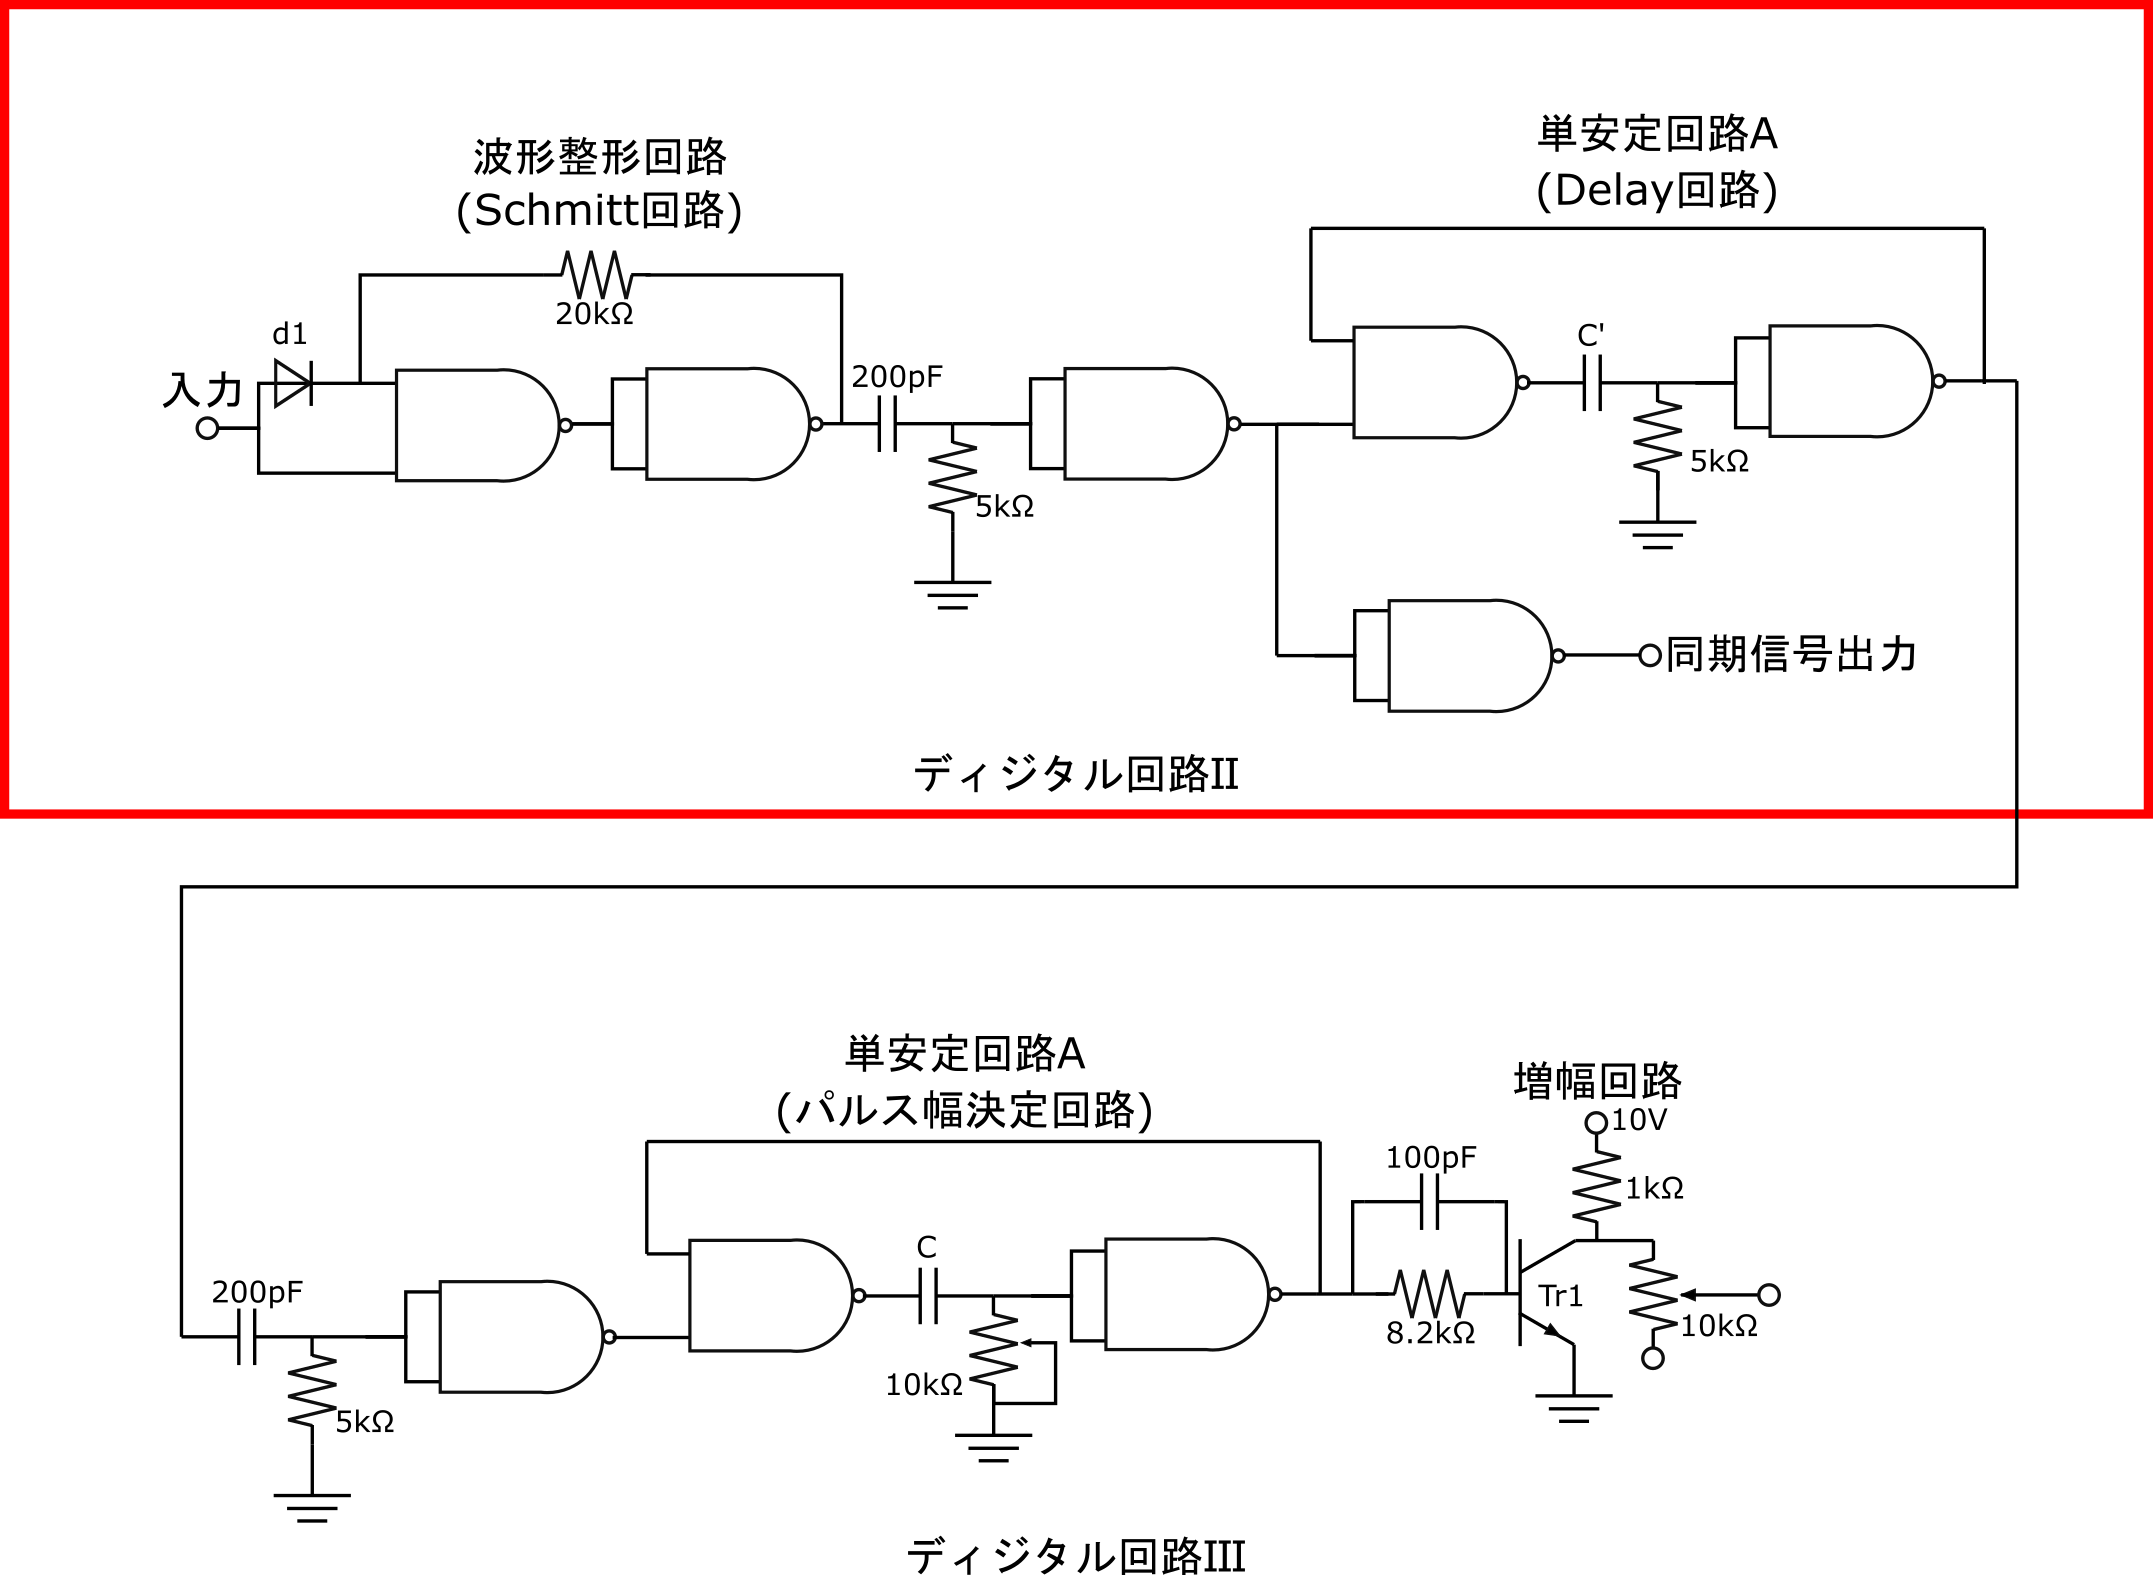
\includegraphics[width=\hsize]{images/text/fig1.png}
	\caption{パルス発生回路}
\end{figure}
\subparagraph{パルス発生回路の入力信号}
図1に示すパルス発生回路の最初の回路である波形整形回路(Schmitt回路)の入力信号には,備品の発振器の出力信号を用いる.出呂波形は正弦波とし,周波数は1kHzを基準とする.

\subsection{NAND回路を2個つないだときの入出力特性}
図2のようにNAND回路を2個つなぎ,入力側の1端子を IC端子の$V_{CC}$用電源$+5V$につなぎ,他端子に可変電流電源を接続して入力でなんつを変化していったときの出力端子の電圧の変化を図のように電子電圧計で測定すると図3のような入出力特性がえられる.
\begin{figure}[H]
  \begin{minipage}{0.5\hsize}
    \centering
   	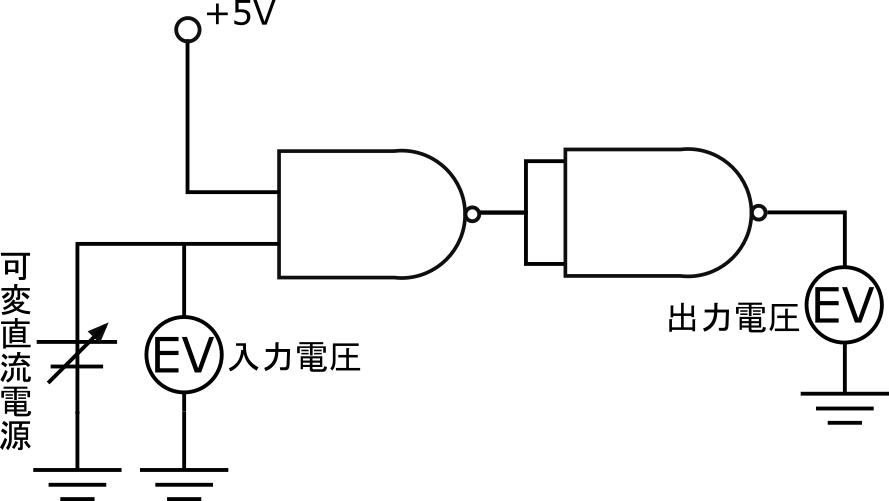
\includegraphics[width=\hsize]{images/text/fig2.png}
    \caption{入出力測定回路}
  \end{minipage}
  \begin{minipage}{0.5\hsize}
    \centering
	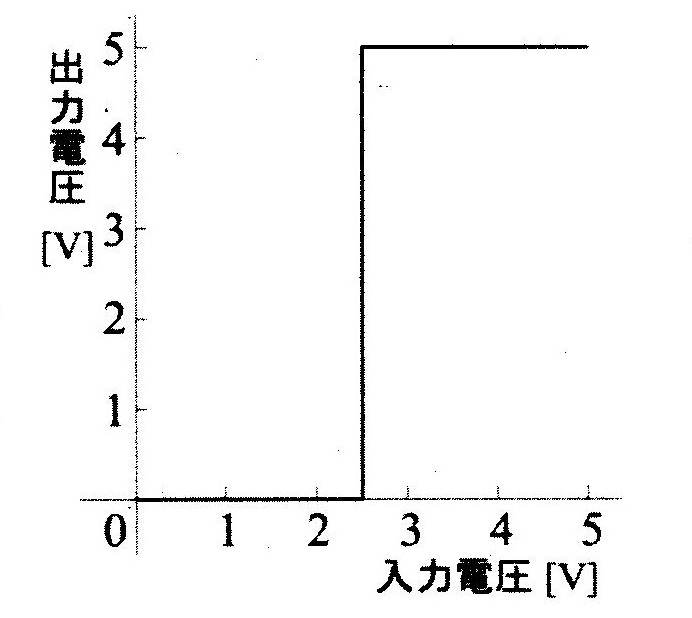
\includegraphics[height=40mm]{images/text/fig3.png}
    \caption{入出力特性}
  \end{minipage}
\end{figure}

\section{実験方法}

\subsection{波形整形回路(Schmitt回路)の静特性の測定}
波形整形回路(Schmitt回路)を,図4の構成により図2の入出力特性の測定と同様,入力の可変電流電源を変化して行ったときの出力電圧の変化すなわち静的な入出力特性を測定する.
図5のような入出力特性(ヒステリシス特性)が得られる.
ヒステリシス特性がどのように変化するか調べる.
\begin{figure}[H]
  \begin{minipage}{0.5\hsize}
    \centering
   	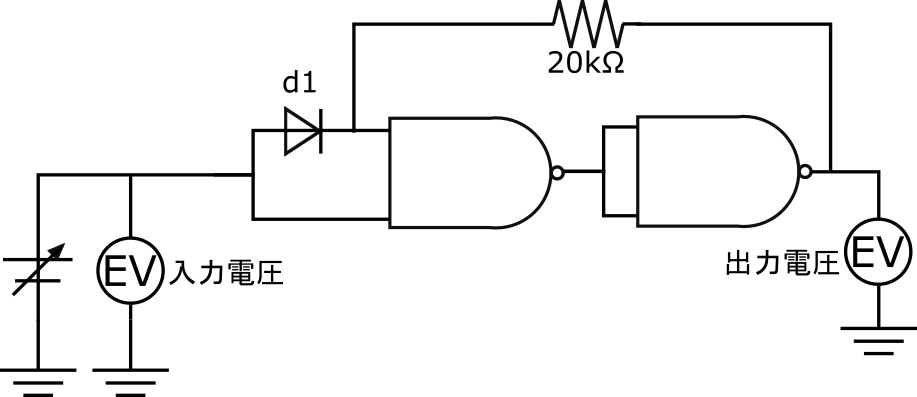
\includegraphics[width=0.9\hsize]{images/text/fig4.png}
    \caption{波形整形回路(Schmitt回路)の静特性測定回路}
  \end{minipage}
  \begin{minipage}{0.5\hsize}
    \centering
	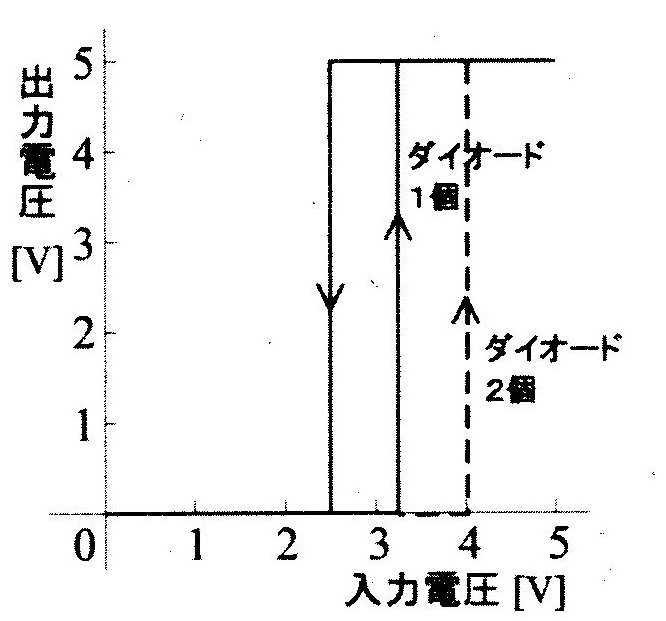
\includegraphics[height=45mm]{images/text/fig5.png}
    \caption{波形整形回路の静特性}
  \end{minipage}
\end{figure}

\newpage
\subsection{波形整形回路(Schmitt回路)の動特性の測定}
図6の構成により,入力信号として発振器により発振周波数1kHzの正弦波を入力し波形整形回路(Schmitt回路)のa,b,c,d各店の波形をオシロスコープで測定する.
図7は正弦波形の入力に対する各部の波形例を示す.測定する時,各店波形の時間軸を必ず揃えておくこと.
さらに,各点の波形は直流で観測すること.
\begin{figure}[H]
  \begin{minipage}{0.5\hsize}
    \centering
   	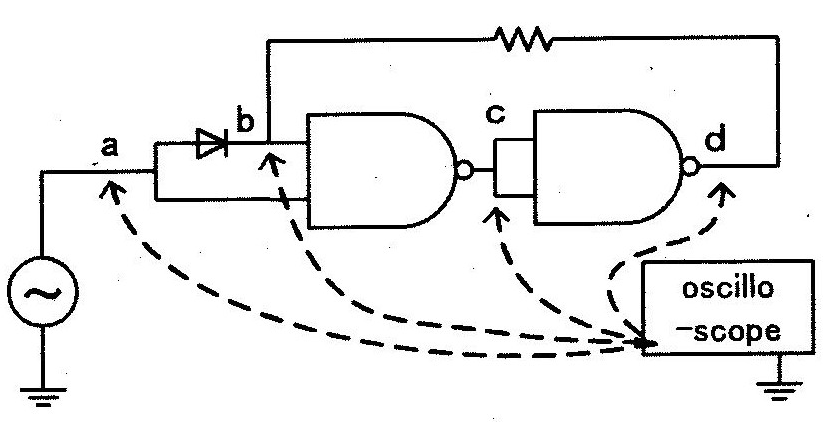
\includegraphics[width=\hsize]{images/text/fig6.png}
    \caption{波形整形回路(Schmitt回路)の動特性測定回路}
  \end{minipage}
  \begin{minipage}{0.5\hsize}
    \centering
	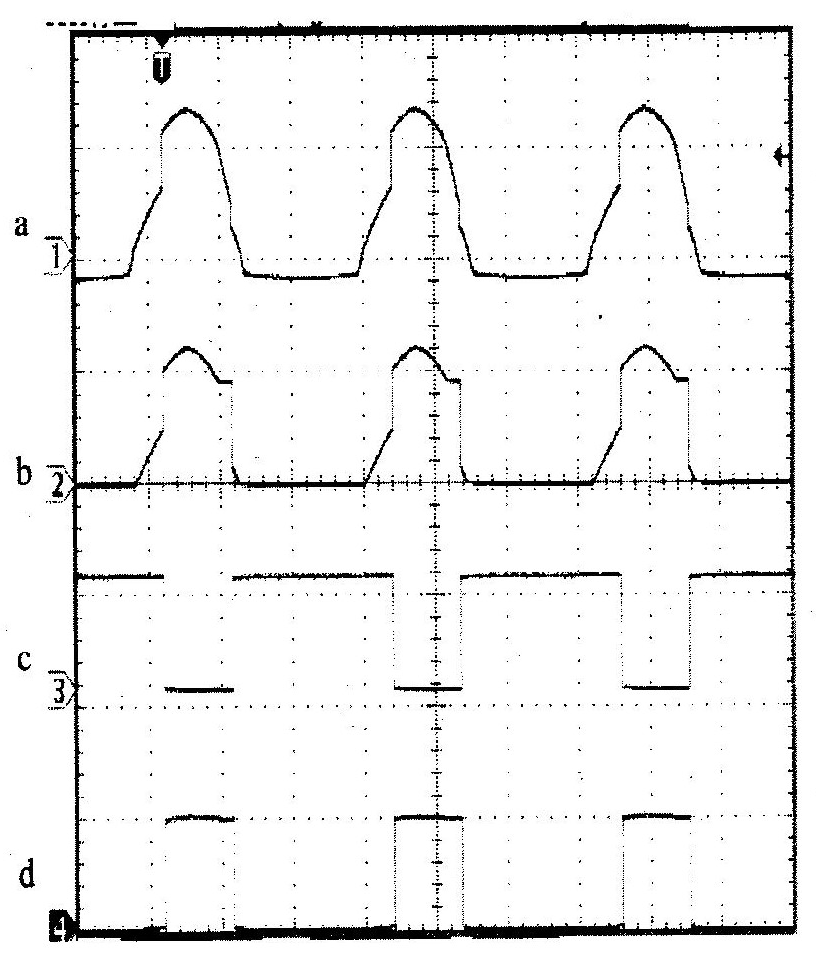
\includegraphics[width=\hsize]{images/text/fig7.png}
    \caption{波形整形回路の各部の波形}
  \end{minipage}
\end{figure}
\subparagraph{同期用信号出力機}
図6の波形整形回路(Schmitt回路)の出力を微分し,それをNAND回路に入れ,その出力を単安定回路A(Delay回路)の入力として,さらに同期用信号としても用いる.
単安定回路A(Delay回路)の出力信号を同期信号でトリガをかけ,オシロスコープで観測する.
このようにすると,同期用信号が観測しようとする単安定回路A(Delay回路)の出力より時間的に先に存在するので,単安定回路A(Delay回路)の出力の様子を確実に観測できる.
\begin{figure}[H]
	\centering
	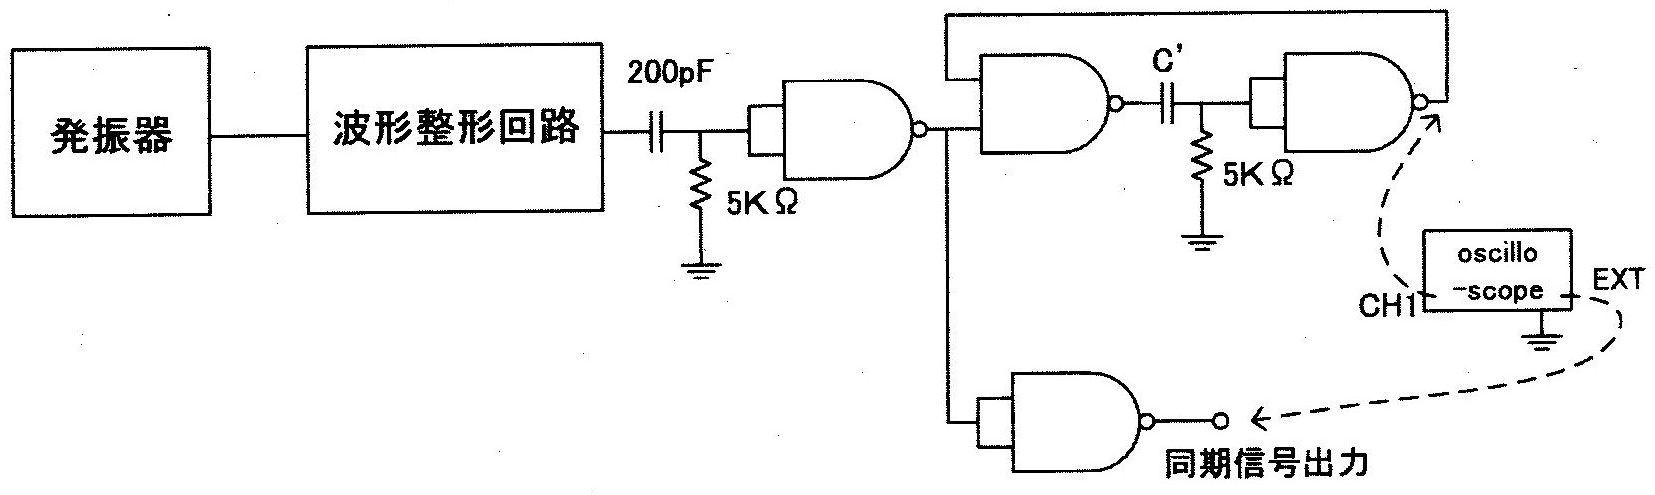
\includegraphics[width=\hsize, height=50mm]{images/text/fig8.png}
	\caption{遅延時間測定回路}
\end{figure}

\newpage
\subsection{遅延回路A(Delay回路)の遅延時間の測定}
図8のような回路を組み立てて容量C'を適当に変えて遅延時間を測定する.
図9にオシロスコープの画面例を,図10に測定結果の一例を示す.
\begin{figure}[H]
  \begin{minipage}{0.5\hsize}
    \centering
   	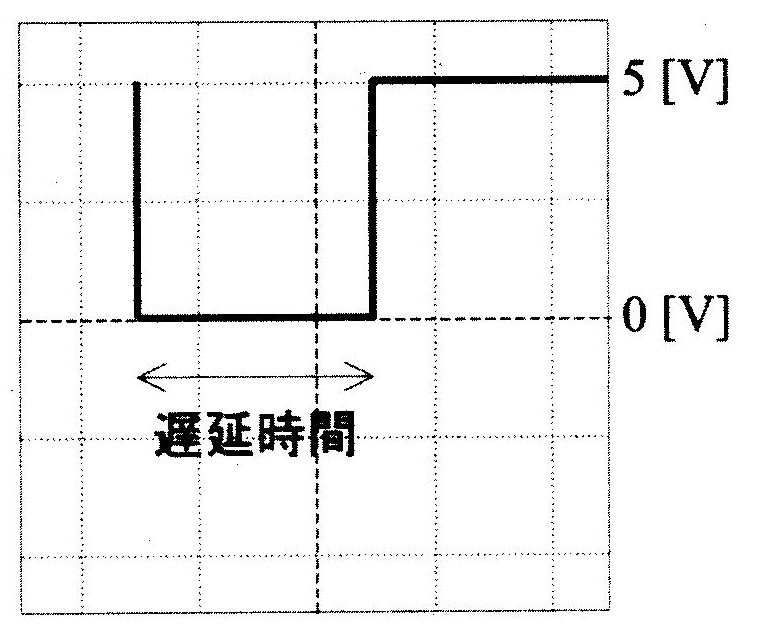
\includegraphics[width=0.7\hsize]{images/text/fig9.png}
    \caption{オシロスコープの画面例}
  \end{minipage}
  \begin{minipage}{0.5\hsize}
    \centering
	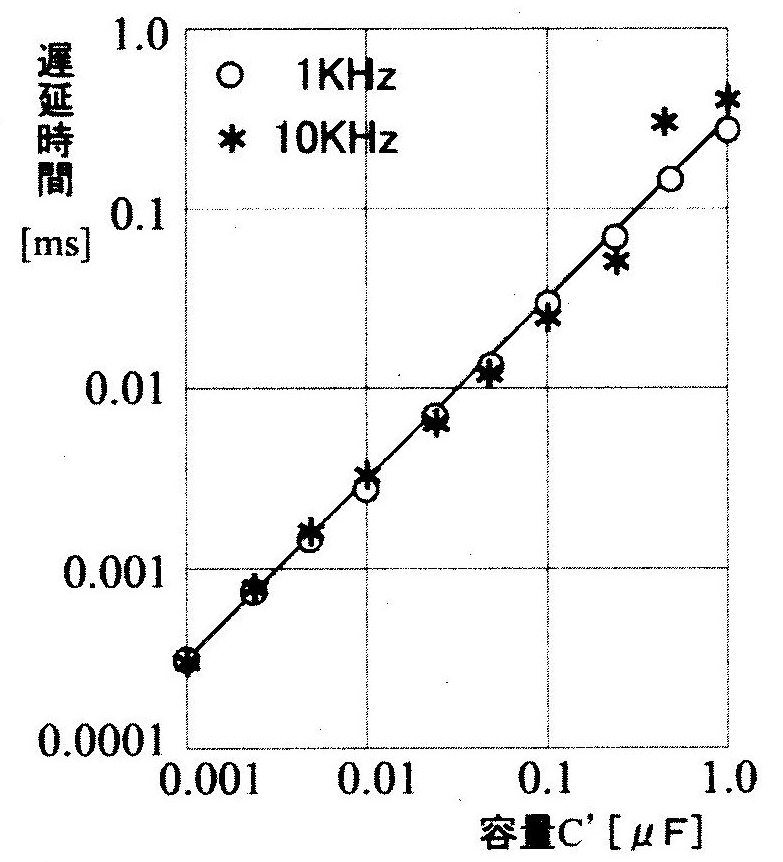
\includegraphics[width=0.7\hsize]{images/text/fig10.png}
    \caption{パルス幅・容量特性}
  \end{minipage}
\end{figure}
ただし,発振器の周波数は$1kHz$および$10kHz$の2種類を測定すること.
測定終了後は,次の実験 ''ディジタル回路3'' で利用するため,遅延時間が$0.01[ms]$となるように容量C'を決定し,回路を変更しておくこと.

\section{使用器具}
今回の実験において,以下の表に示す器具を用いて測定を行った.
\begin{figure}[H]
	\centering
	\tblcaption{使用器具}
	\label{tbl:使用器具}
	\begin{tabular}{|c|c|c|}\hline
		使用器具名 & 型番 & 管理番号等 \\\hline
		ディジタルオシロスコープ & DSO3062A & BH43H17S00000021 \\\hline
		多出力直流安定化電源 & PW26-1AT & 20"と書いた黄色いシールのあるもの \\\hline
		直流安定化電源 & PR18-1.2A & い 102 383 \\\hline
		直流電圧計 & 2051-05 & い 54 102 \\\hline
		低周波発振器 & AG-203E & 20"と書いた黄色いシールのあるもの \\\hline
		デジタル・マルチメータ & VOAC86A & 20"と書いた赤いシールのあるもの \\\hline
	\end{tabular}
\end{figure}

\newpage
\section{実験結果}
\subsection{波形整形回路(Schmitt回路)の静特性の測定}
図\ref{fig:5.1.1.circuit},\ref{fig:5.1.2.circuit}に示す回路図の回路を図\ref{fig:5.1.1.camera},\ref{fig:5.1.2.camera}のように作成し,3.1に示した実験を行った.
その測定値を表\ref{tbl:5.1.1},\ref{tbl:5.1.2},\ref{tbl:5.1.3},\ref{tbl:5.1.4}に,測定値を元に入力電圧と出力電圧の関係を図\ref{fig:5.2.graph}に示す.
\begin{figure}[H]
  \begin{minipage}{0.5\hsize}
    \centering
    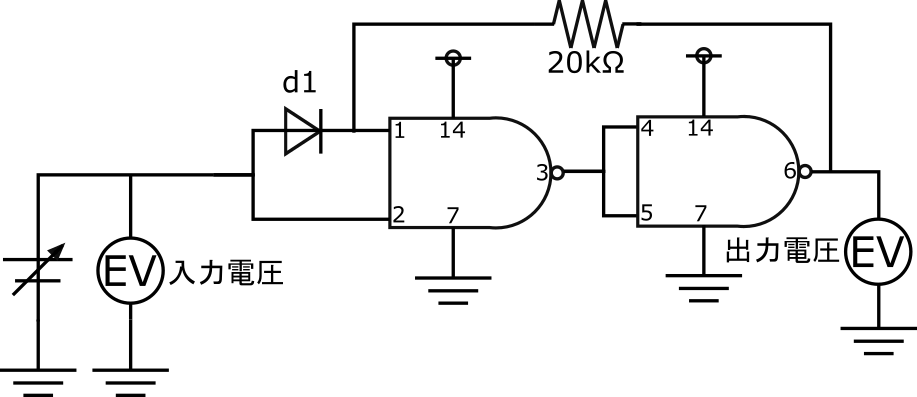
\includegraphics[width=0.9\hsize]{images/Experiment/5_1_1_circuit.png}
    \figcaption{ダイオード1個・昇圧時の測定回路}
	\label{fig:5.1.1.circuit}
  \end{minipage}
  \begin{minipage}{0.5\hsize}
    \centering
    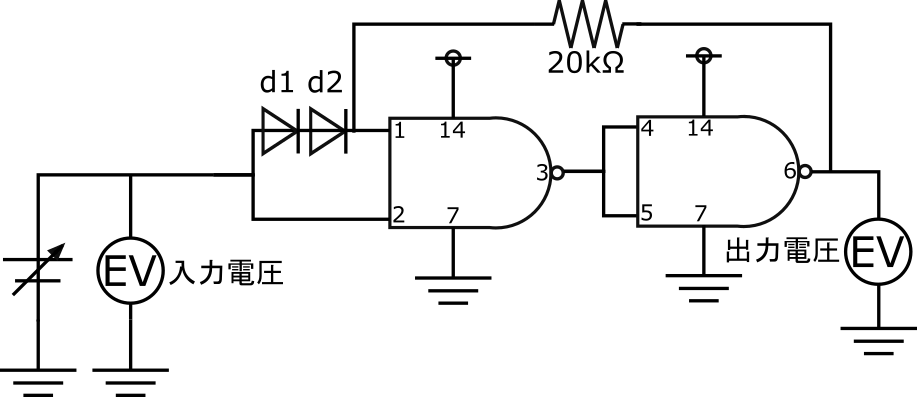
\includegraphics[width=0.9\hsize]{images/Experiment/5_1_2_circuit.png}
    \caption{ダイオード2個・昇圧時の測定回路}
	\label{fig:5.1.2.circuit}
  \end{minipage}
\end{figure}
\begin{figure}[H]
  \begin{minipage}{0.5\hsize}
    \centering
    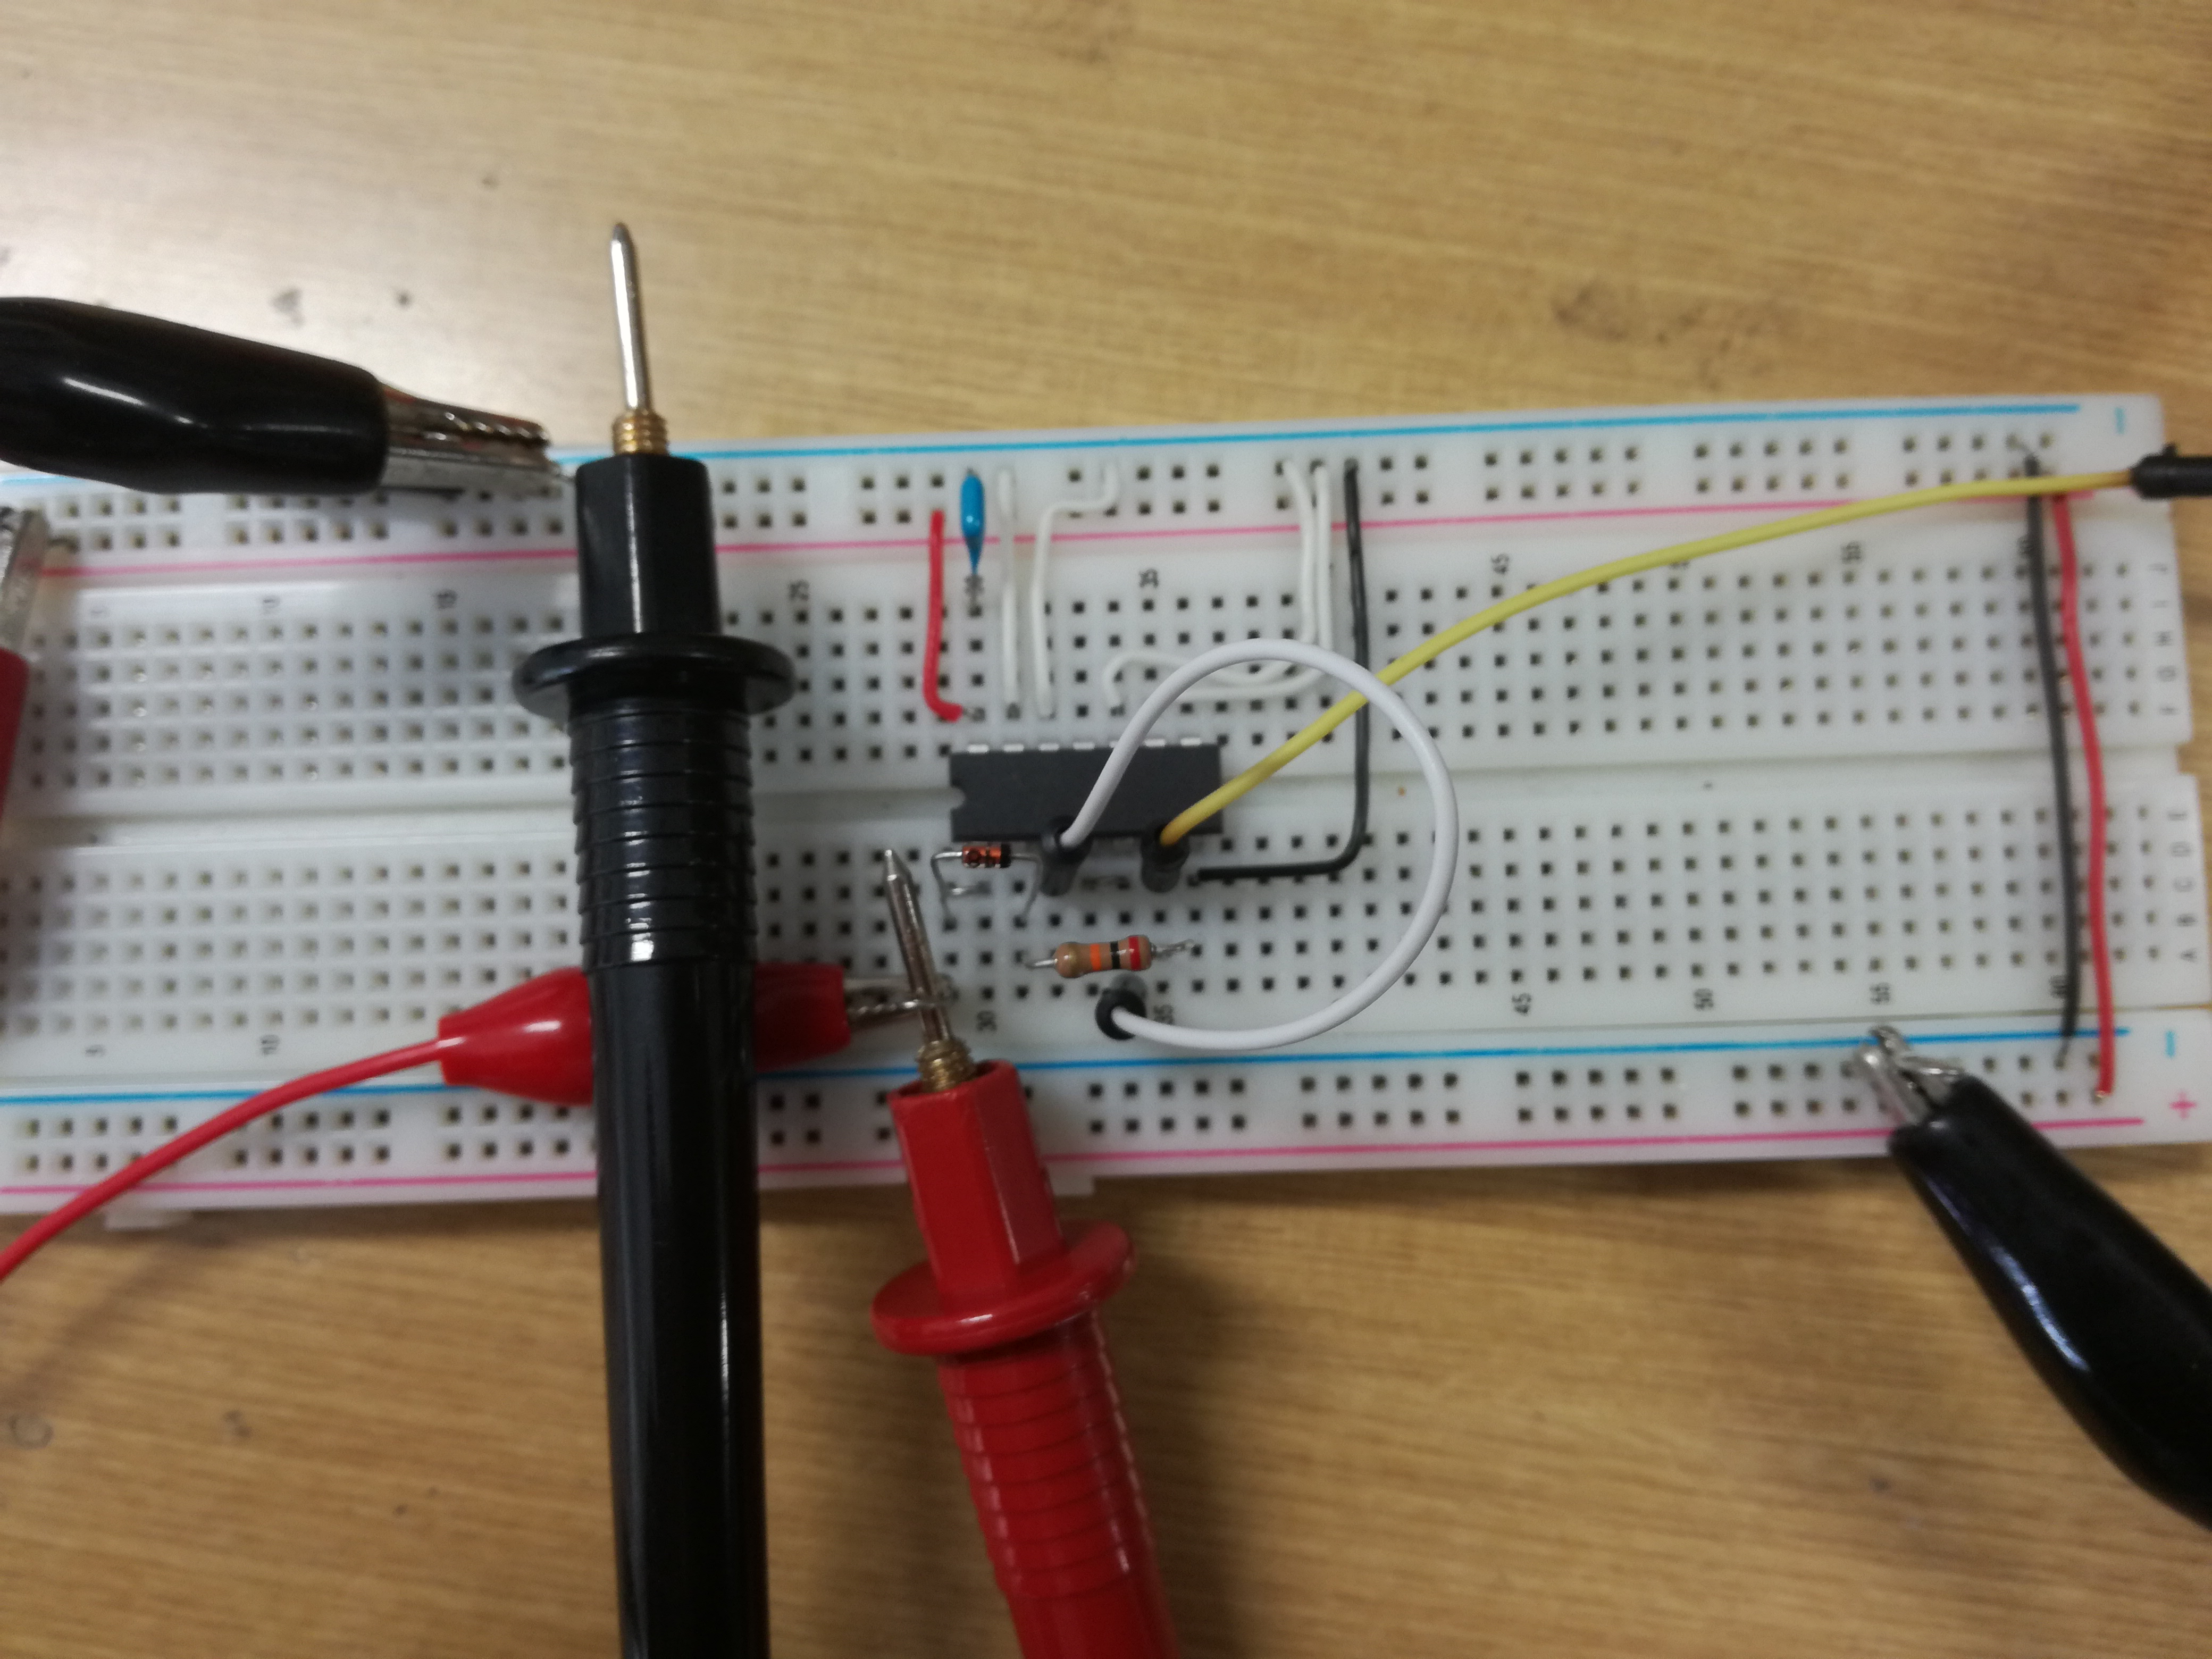
\includegraphics[width=0.9\hsize]{images/camera/5_1_1_camera.jpg}
    \figcaption{ダイオード1個・昇圧時の測定回路}
	\label{fig:5.1.1.camera}
  \end{minipage}
  \begin{minipage}{0.5\hsize}
    \centering
    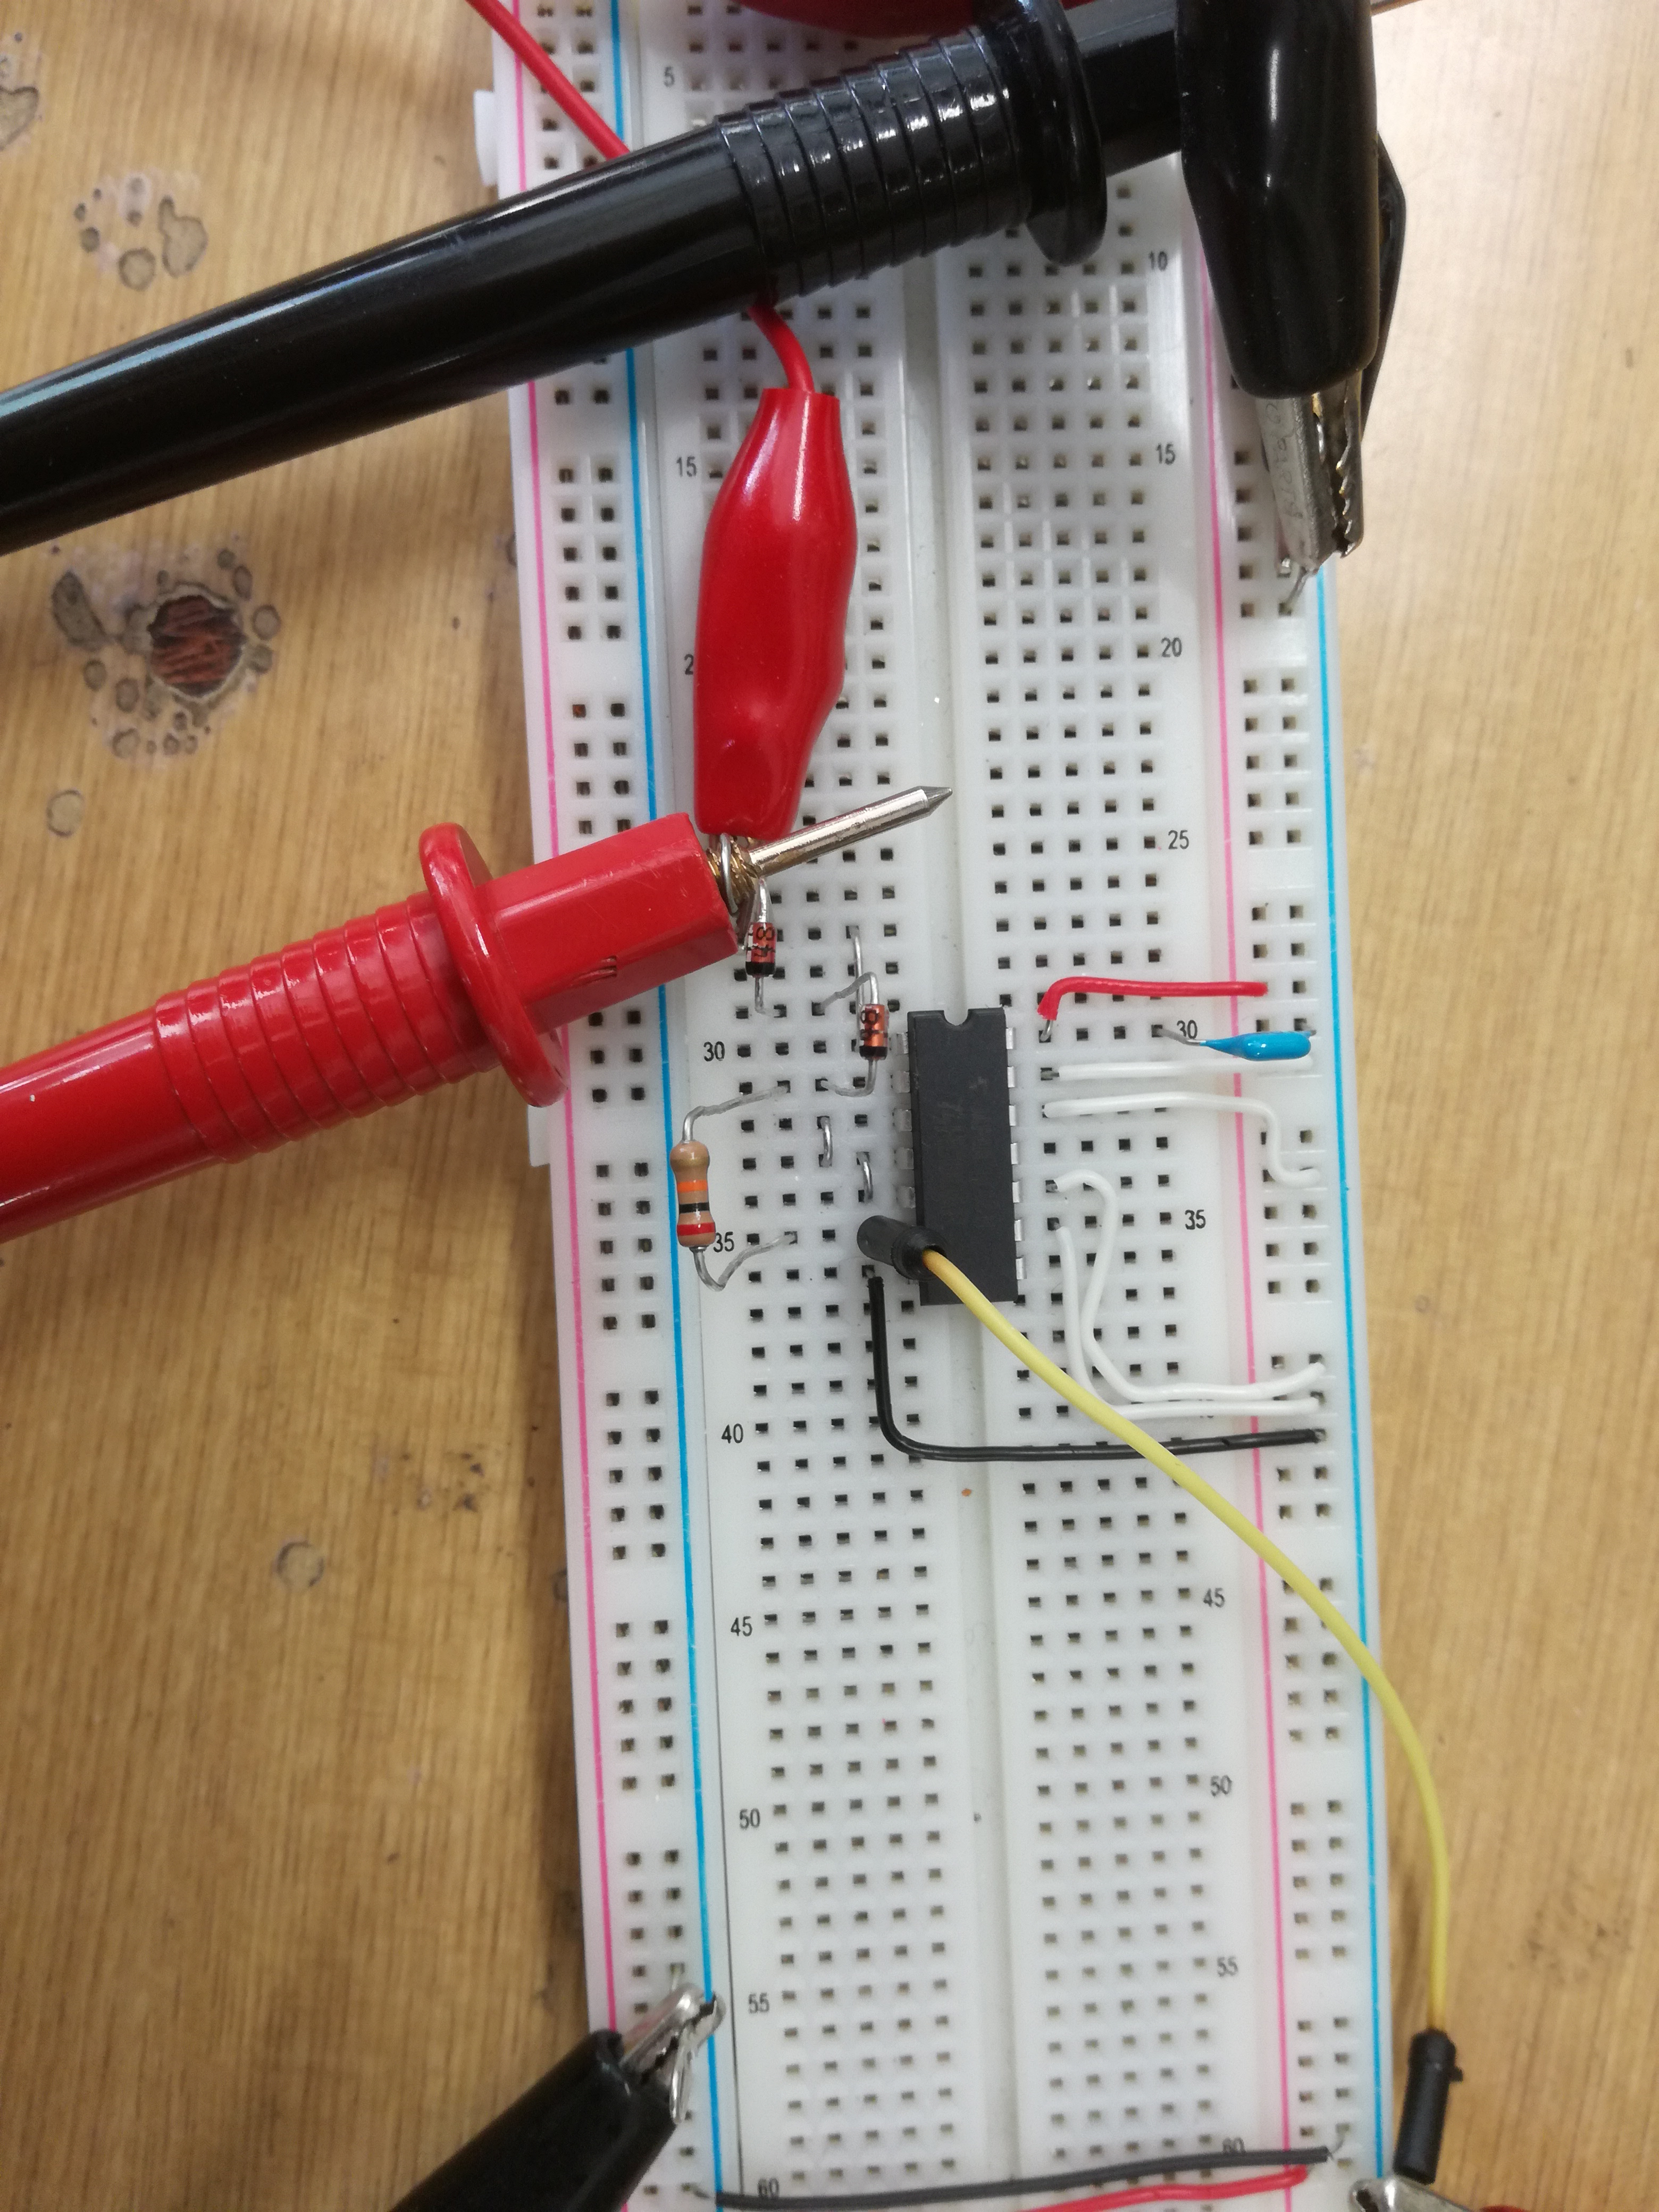
\includegraphics[height=0.9\hsize, angle=270]{images/camera/5_1_2_camera.jpg}
    \caption{ダイオード2個・昇圧時の測定回路}
	\label{fig:5.1.2.camera}
  \end{minipage}
\end{figure}
\begin{figure}[H]
	\begin{tabular}{cc}
		\begin{minipage}{0.5\hsize}
			\tblcaption{ダイオード1個・昇圧時の測定値}
			\label{tbl:5.1.1}
			\centering
			\small
			\begin{tabular}{|c|c|}\hline
				入力電圧[V] & 出力電圧[V] \\\hline
				0.000 & 0.000 \\\hline
				0.200 & 0.000 \\\hline
				0.401 & 0.000 \\\hline
				0.601 & 0.000 \\\hline
				0.801 & 0.000 \\\hline
				1.001 & 0.001 \\\hline
				1.201 & 0.002 \\\hline
				1.401 & 0.003 \\\hline
				1.602 & 0.004 \\\hline
				1.802 & 0.006 \\\hline
				2.002 & 0.009 \\\hline
				2.202 & 0.013 \\\hline
				2.402 & 0.017 \\\hline
				2.602 & 0.022 \\\hline
				2.802 & 0.026 \\\hline
				3.003 & 0.032 \\\hline
				3.052 & 0.037 \\\hline
				3.103 & 0.046 \\\hline
				3.153 & 0.065 \\\hline
				3.203 & 5.020 \\\hline
				3.403 & 5.020 \\\hline
				3.603 & 5.020 \\\hline
				3.803 & 5.020 \\\hline
				4.003 & 5.020 \\\hline
				4.205 & 5.020 \\\hline
				4.404 & 5.020 \\\hline
				4.604 & 5.020 \\\hline
				4.804 & 5.020 \\\hline
				5.002 & 5.020 \\\hline
			\end{tabular}
			\normalsize
		\end{minipage}
		\begin{minipage}{0.5\hsize}
			\tblcaption{ダイオード1個・降圧時の測定値}
			\label{tbl:5.1.2}
			\centering
			\small
			\begin{tabular}{|c|c|}\hline
				入力電圧[V] & 出力電圧[V] \\\hline
				5.003  & 5.020  \\\hline
				4.804  & 5.020  \\\hline
				4.602  & 5.020  \\\hline
				4.402  & 5.020  \\\hline
				4.202  & 5.020  \\\hline
				4.003  & 5.020  \\\hline
				3.803  & 5.020  \\\hline
				3.603  & 5.020  \\\hline
				3.403  & 5.020  \\\hline
				3.203  & 5.020  \\\hline
				3.002  & 5.020  \\\hline
				2.803  & 5.020  \\\hline
				2.602  & 5.020  \\\hline
				2.402  & 5.020  \\\hline
				2.302  & 0.015  \\\hline
				2.202  & 0.013  \\\hline
				2.002  & 0.009  \\\hline
				1.802  & 0.006  \\\hline
				1.602  & 0.004  \\\hline
				1.402  & 0.003  \\\hline
				1.201  & 0.002  \\\hline
				1.001  & 0.001  \\\hline
				0.801  & 0.001  \\\hline
				0.601  & 0.000  \\\hline
				0.401  & 0.000  \\\hline
				0.200  & 0.000  \\\hline
				0.000  & 0.000  \\\hline
			\end{tabular}
			\normalsize
		\end{minipage}
	\end{tabular}
\end{figure}
\begin{figure}[H]
	\begin{tabular}{cc}
		\begin{minipage}{0.5\hsize}
			\tblcaption{ダイオード2個・昇圧時の測定値}
			\label{tbl:5.1.3}
			\centering
			\small
			\begin{tabular}{|c|c|}\hline
				入力電圧[V] & 出力電圧[V] \\\hline
				0.000 & 0.000 \\\hline
				0.200 & 0.000 \\\hline
				0.400 & 0.000 \\\hline
				0.601 & 0.000 \\\hline
				0.801 & 0.000 \\\hline
				1.001 & 0.000 \\\hline
				1.201 & 0.001 \\\hline
				1.401 & 0.001 \\\hline
				1.602 & 0.002 \\\hline
				1.802 & 0.002 \\\hline
				2.002 & 0.003 \\\hline
				2.202 & 0.004 \\\hline
				2.402 & 0.005 \\\hline
				2.602 & 0.007 \\\hline
				2.802 & 0.009 \\\hline
				3.002 & 0.011 \\\hline
				3.203 & 0.014 \\\hline
				3.403 & 0.020 \\\hline
				3.453 & 5.020 \\\hline
				3.503 & 5.020 \\\hline
				3.603 & 5.020 \\\hline
				3.803 & 5.020 \\\hline
				4.003 & 5.020 \\\hline
				4.200 & 5.020 \\\hline
				4.402 & 5.020 \\\hline
				4.603 & 5.020 \\\hline
				4.803 & 5.020 \\\hline
				5.002 & 5.020 \\\hline
			\end{tabular}
			\normalsize
		\end{minipage}
		\begin{minipage}{0.5\hsize}
			\tblcaption{ダイオード2個・降圧時の測定値}
			\label{tbl:5.1.4}
			\centering
			\small
			\begin{tabular}{|c|c|}\hline
				入力電圧[V] & 出力電圧[V] \\\hline
				5.002 & 5.020 \\\hline
				4.803 & 5.020 \\\hline
				4.603 & 5.020 \\\hline
				4.402 & 5.020 \\\hline
				4.200 & 5.020 \\\hline
				4.003 & 5.020 \\\hline
				3.803 & 5.020 \\\hline
				3.603 & 5.020 \\\hline
				3.407 & 5.020 \\\hline
				3.203 & 5.020 \\\hline
				3.002 & 5.020 \\\hline
				2.803 & 5.020 \\\hline
				2.602 & 5.020 \\\hline
				2.402 & 5.020 \\\hline
				2.352 & 0.005 \\\hline
				2.307 & 0.005 \\\hline
				2.202 & 0.004 \\\hline
				2.002 & 0.003 \\\hline
				1.802 & 0.002 \\\hline
				1.601 & 0.002 \\\hline
				1.401 & 0.001 \\\hline
				1.201 & 0.001 \\\hline
				1.003 & 0.000 \\\hline
				0.801 & 0.000 \\\hline
				0.601 & 0.000 \\\hline
				0.401 & 0.000 \\\hline
				0.201 & 0.000 \\\hline
				0.000 & 0.000 \\\hline
			\end{tabular}
			\normalsize
		\end{minipage}
	\end{tabular}
\end{figure}
\begin{figure}[H]
	\centering
	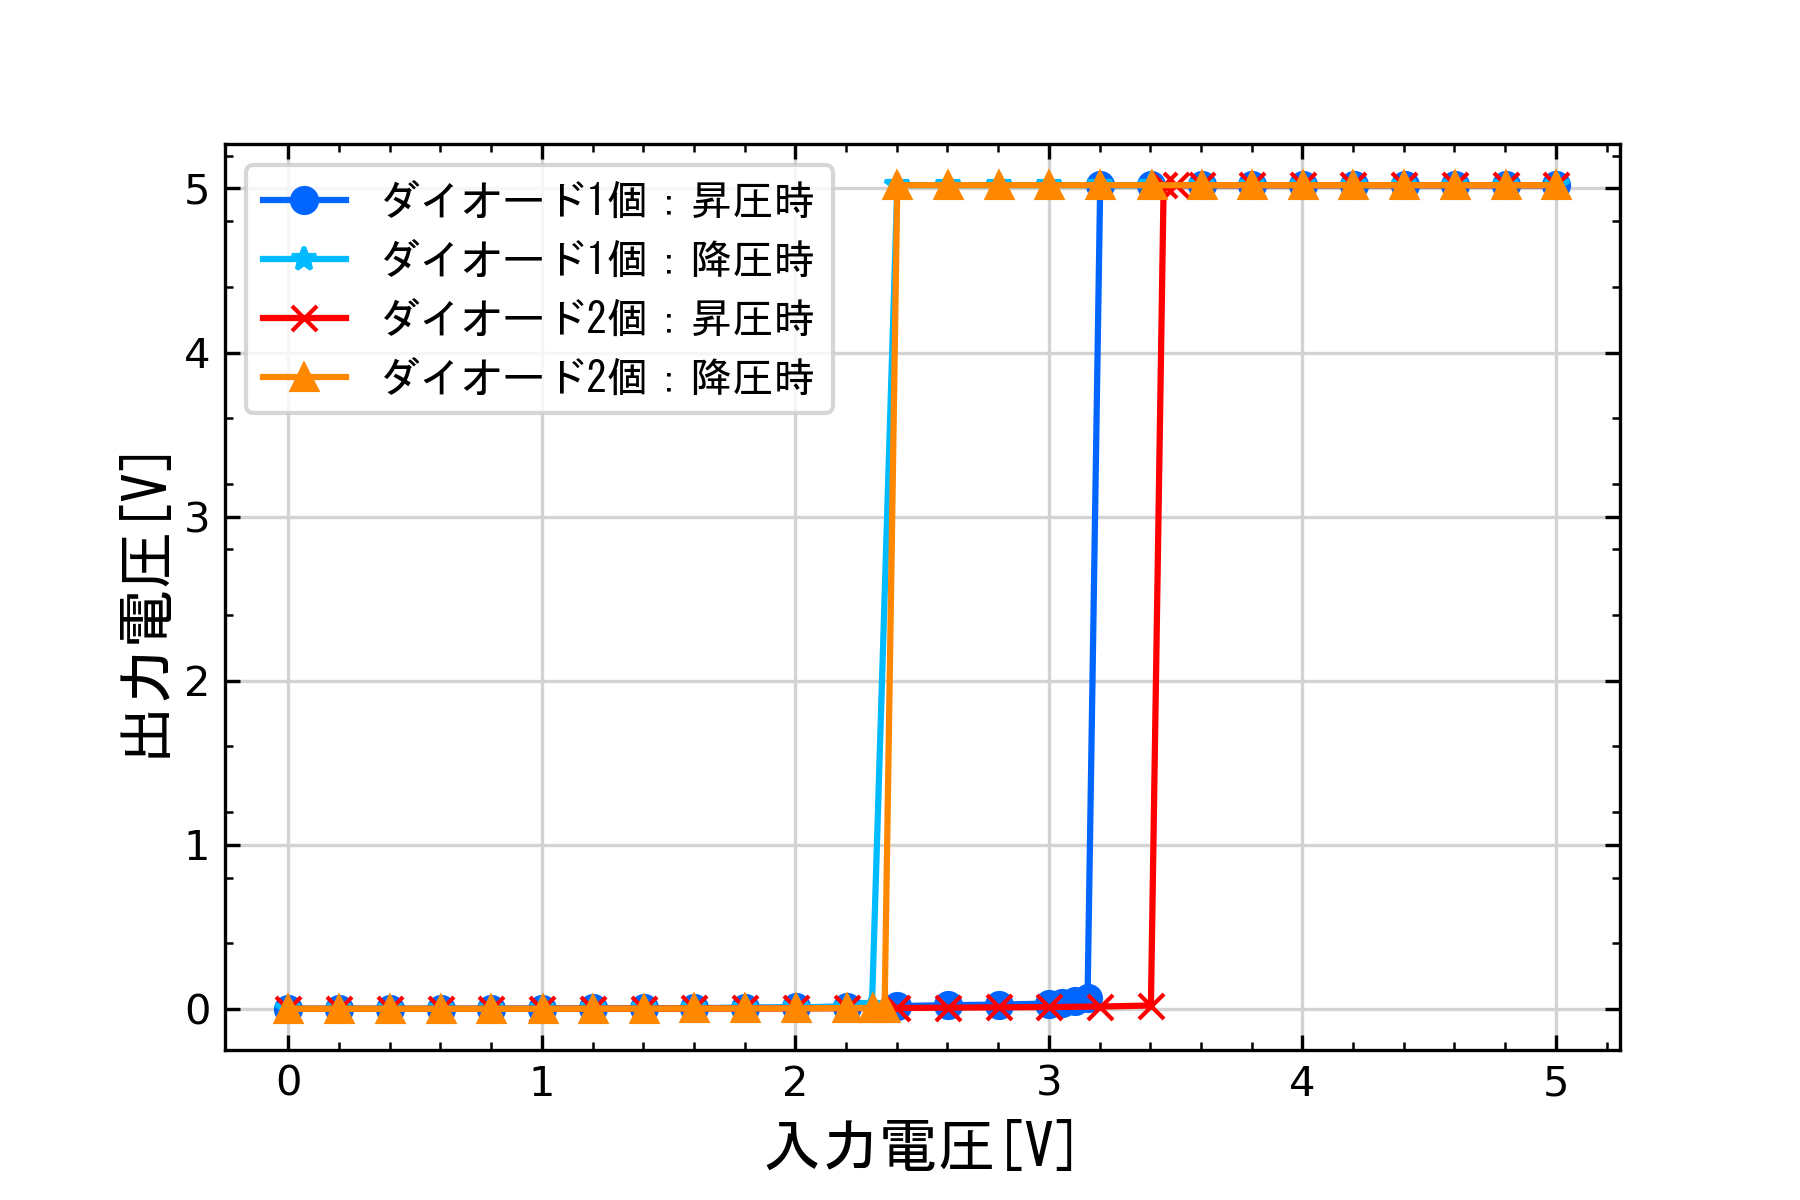
\includegraphics[height=80mm]{images/Experiment/5_1_graph.png}
	\caption{波形整形回路の静特性}
	\label{fig:5.1.graph}
\end{figure}

\subsection{波形整形回路(Schumitt回路)の動特性の測定}
3.2に示した実験を,図\ref{fig:5.1.1.circuit}に示した回路を用いて行った.
デジタルオシロスコープを用いて測定した電圧波形を以下の図\ref{fig:5.2.graph}に示す.
\begin{figure}[H]
	\centering
	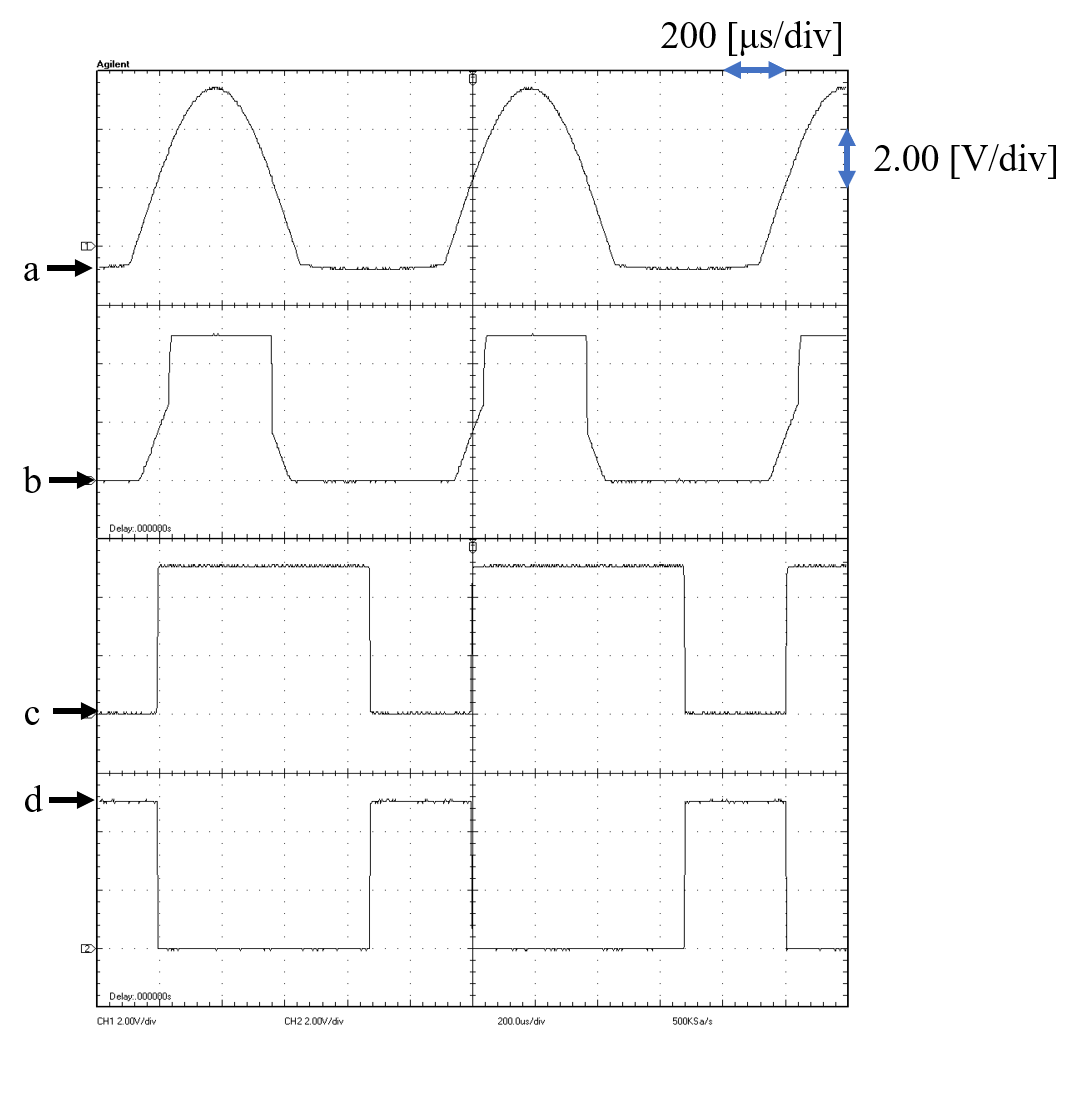
\includegraphics[height=120mm]{images/Experiment/5_2_graph.png}
	\caption{波形整形回路の各部波形}
	\label{fig:5.2.graph}
\end{figure}

\newpage
\subsection{遅延回路A(Delay)回路の遅延時間の測定}
図\ref{fig:5.3.circuit}に示す回路図の回路を図\ref{fig:5.3.camera}のように作成し,3.3に示す実験を行った.
測定した静電容量と遅延時間の関係を表\ref{tbl:5.3.data}に示す測定値をもとに図\ref{fig:5.3.graph}に示す.
\begin{figure}[H]
	\centering
	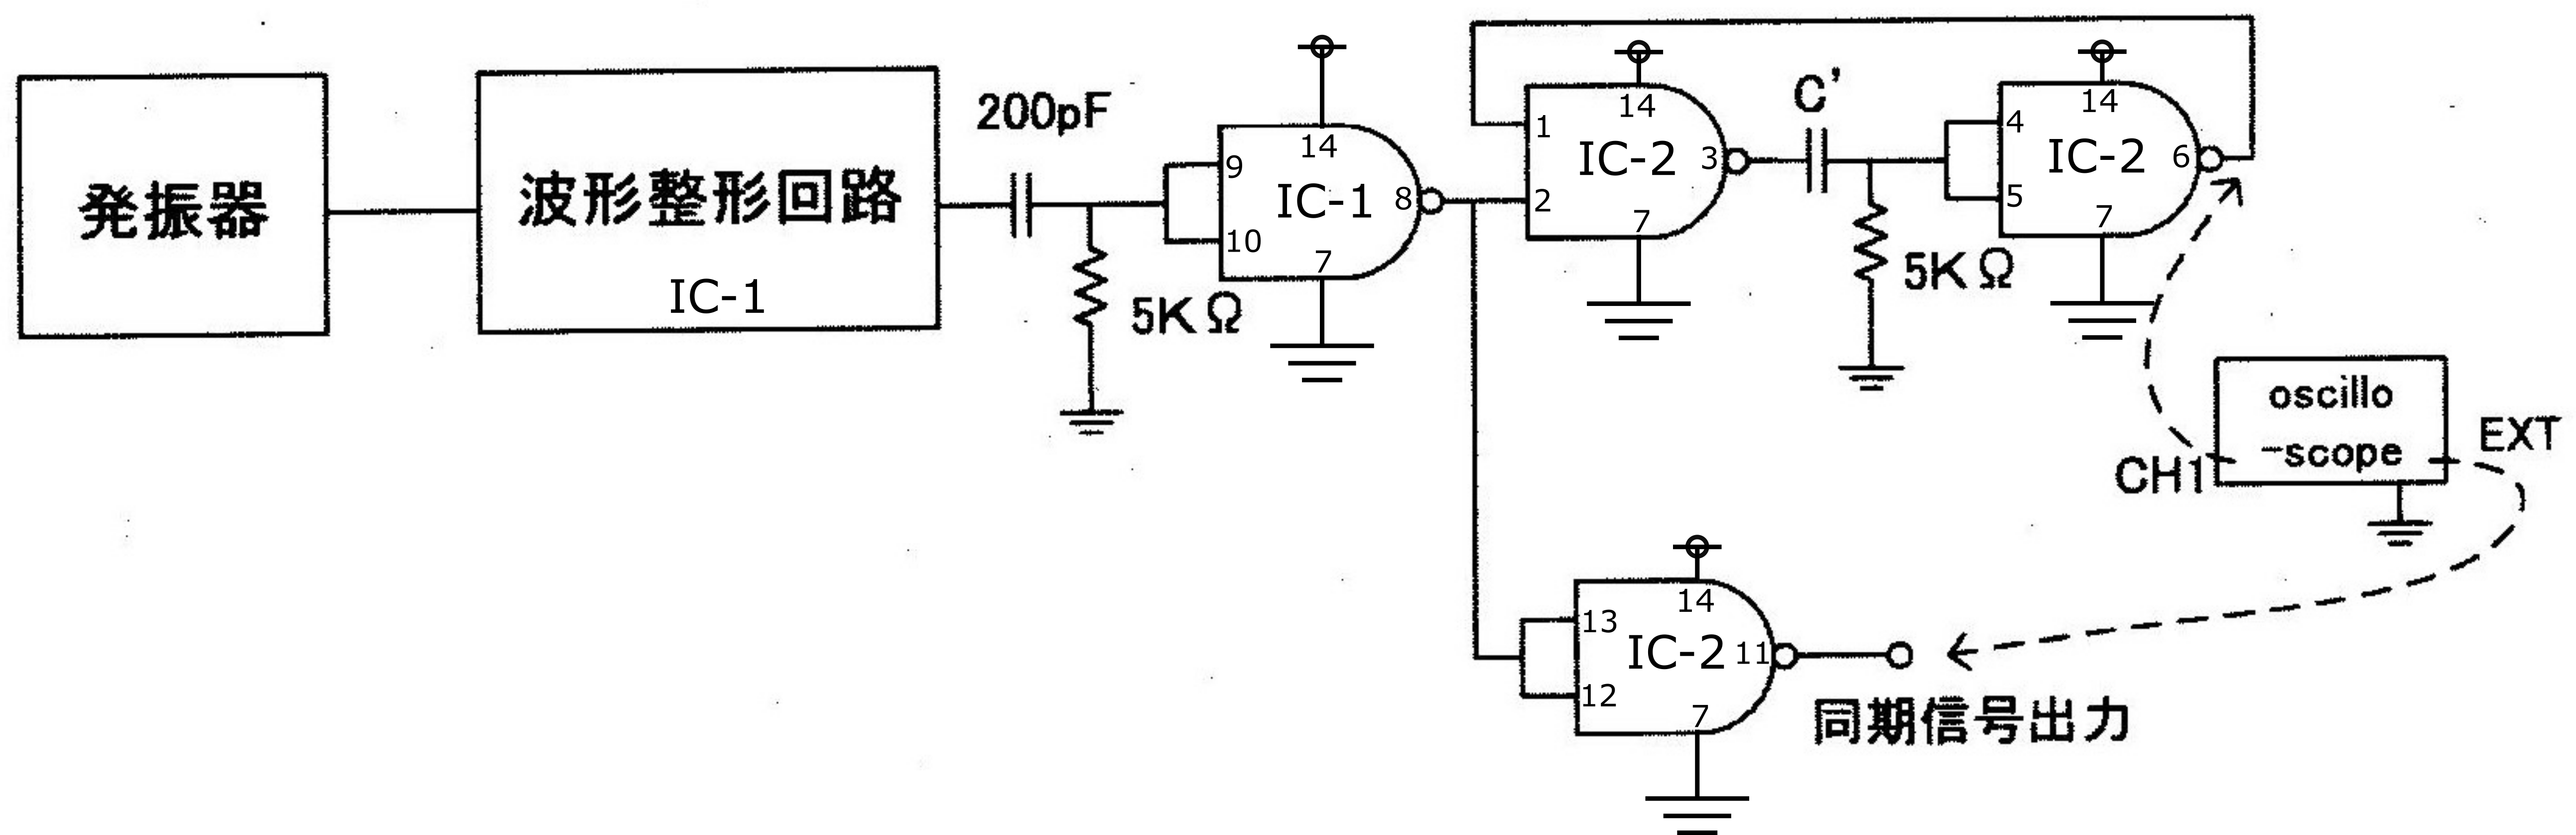
\includegraphics[width=\hsize]{images/Experiment/5_3_circuit.png}
	\caption{制作した測定回路図}
	\label{fig:5.3.circuit}
\end{figure}
\begin{figure}[H]
    \centering
	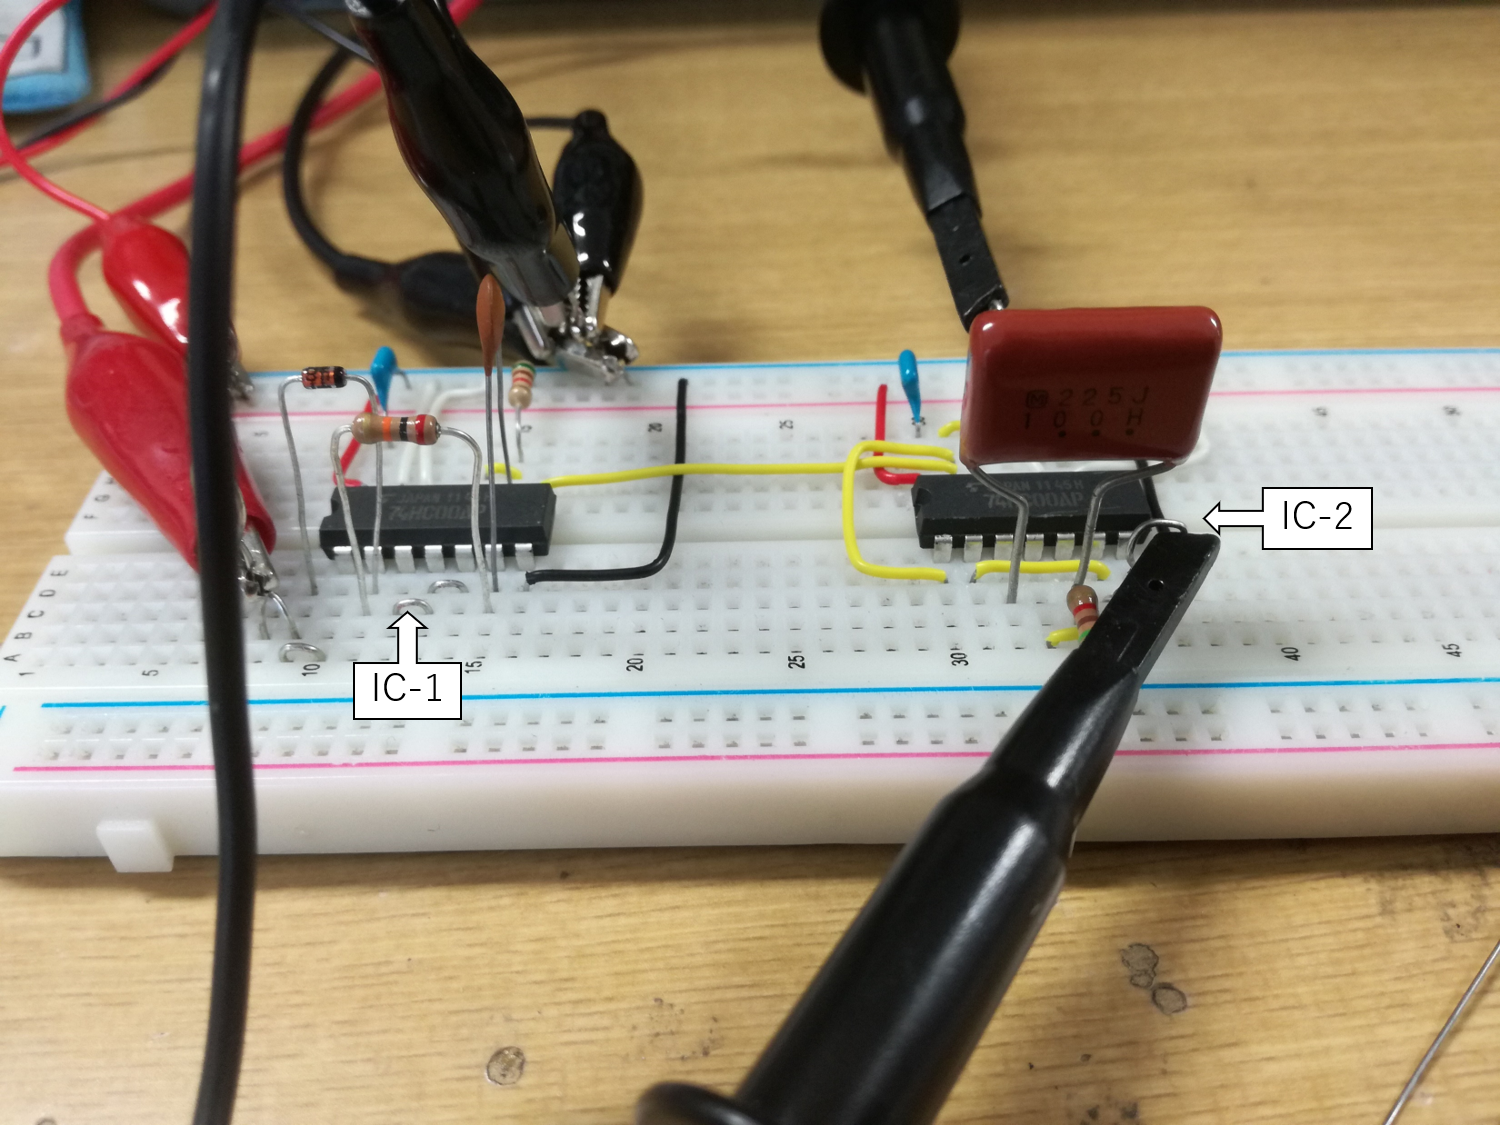
\includegraphics[width=\hsize]{images/camera/5_3_camera.png}
    \caption{制作した測定回路}
	\label{fig:5.3.camera}
\end{figure}
\begin{figure}[H]
	\centering
	\tblcaption{測定値}
	\label{}
	\begin{tabular}{|c|c|c|}\hline
		 & 周波数=1[kHz] & 周波数=10[kHz] \\\cline{2-3}
		容量C'[μF] & \multicolumn{2}{|c|}{遅延時間[ms]}   \\\hline
		2.20.E-10 & 6.00.E-07 & 6.00.E-07 \\\hline
		2.20.E-09 & 6.60.E-06 & 8.00.E-06 \\\hline
		2.20.E-08 & 6.00.E-05 & 5.20.E-05 \\\hline
		2.20.E-07 & 5.00.E-04 & 4.50.E-04 \\\hline
		2.20.E-06 & 4.60.E-03 & 4.60.E-03 \\\hline
	\end{tabular}
\end{figure}
\begin{figure}[H]
	\centering
	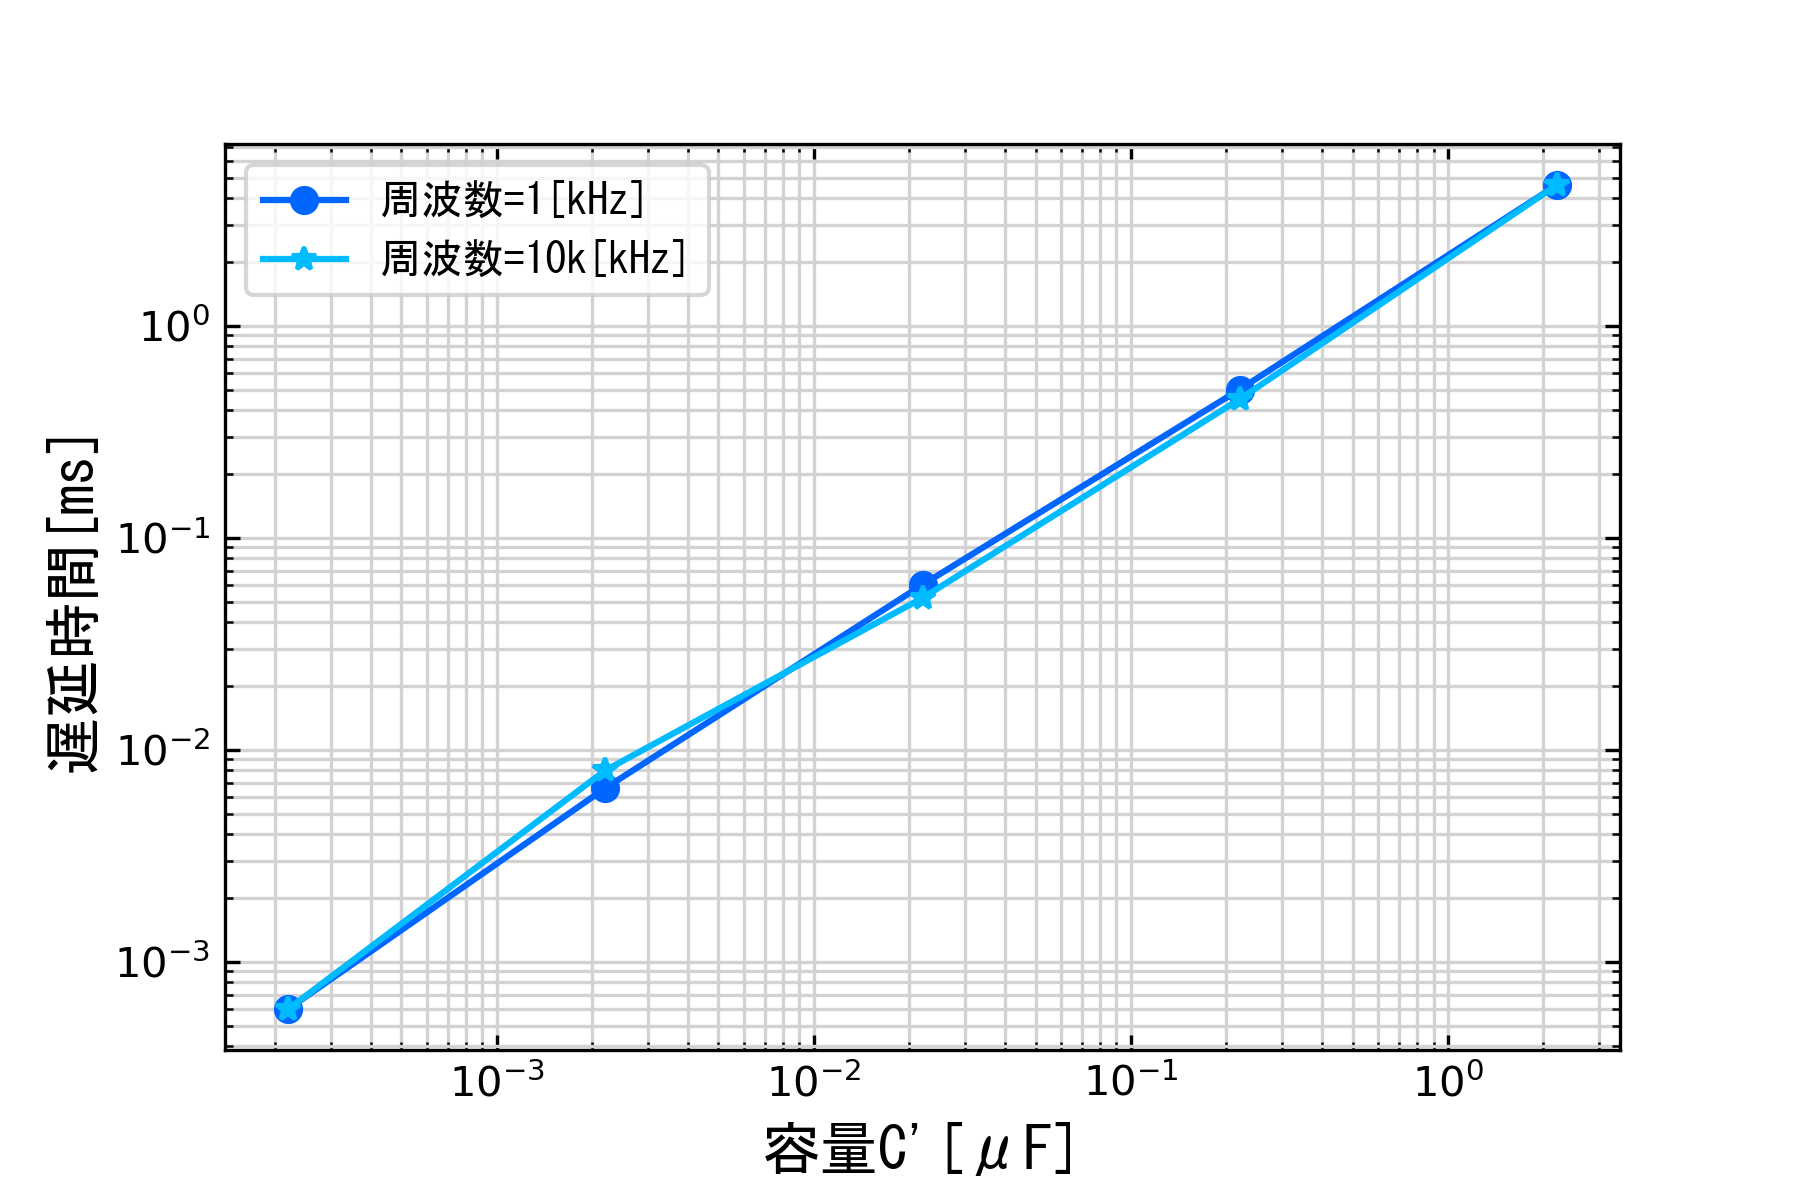
\includegraphics[width=0.9\hsize]{images/Experiment/5_3_graph.png}
	\caption{静電容量と遅延時間の関係}
	\label{fig:5.3.graph}
\end{figure}


\newpage
\section{考察}
\subsection{波形整形回路(Schmitt回路)の静特性の測定}
図\ref{fig:5.1.graph}を見ると,電圧を上げていったときの特性はダイオードの個数によって影響があることがわかる.
これは,ダイオードの個数が増えたことによって,電圧降下が増えたことによるものだと思われる.
このことが電圧を下げていったときに影響が少ないのはダイオードのそのものの特性により,逆電流が流れにくいためであると考えられる.
\subsection{波形整形回路(Schumitt回路)の動特性の測定}
図\ref{fig:5.2.graph}に示した測定結果より,それぞれの波形の意味を考察する.\\
\\
まず,発振器より交流波形が入力される.\\
↓\\
ダイオードで整流された電圧波形(a)が現れる.\\
↓\\
(a)に(d)の波形が合成され(b)の波形が現れる.\\
↓\\
(b)の波形のうち入力電圧がHIGHと認識されない部分が取り除かれ,NOTされて(c)の波形が出力される.\\
↓\\
(c)の波形がNOTされて(d)の波形が出力される.\\
\subsection{遅延回路A(Delay)回路の遅延時間の測定}
図\ref{fig:5.3.graph}に示した静電容量と遅延時間の関係より,これらの値にはべき関数的な関係があることがわかる.


\newpage
\section{吟味事項}
\subsection{図2に示す入出力測定回路において,入力信号がどのような形をしていようとも,例えば正弦波であっても,NAND回路の電圧伝達特性よりNAND出力には常に理想的な短形波が得られると考えられるが,実際はそうならない.どのような波形が出力されるか,またなぜそのような波形になるのか,図2の可変直流電源の代わりに発振器(100Hz程度)を用いて正弦波を入力した時の各部の波形の観察結果をもとに説明せよ.}
以下,図\ref{fig:7.1.circuit},\ref{fig:7.1.camera}にそれぞれ使用した回路図その実際の回路,図\ref{fig:7.1.graph}に100Hz程度の正弦波を入力したときの各部波形を示す.
\begin{figure}[H]
 	\begin{minipage}{0.5\hsize}
    	\centering
   		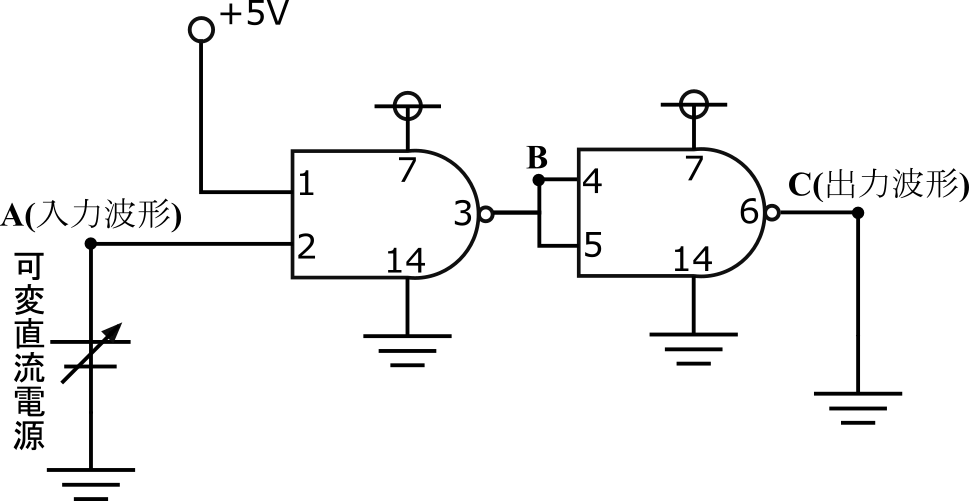
\includegraphics[width=\hsize]{images/Experiment/7_1_circuit.png}
		\caption{測定回路}
		\label{fig:7.1.circuit}
	\end{minipage}
	\begin{minipage}{0.5\hsize}
    	\centering
		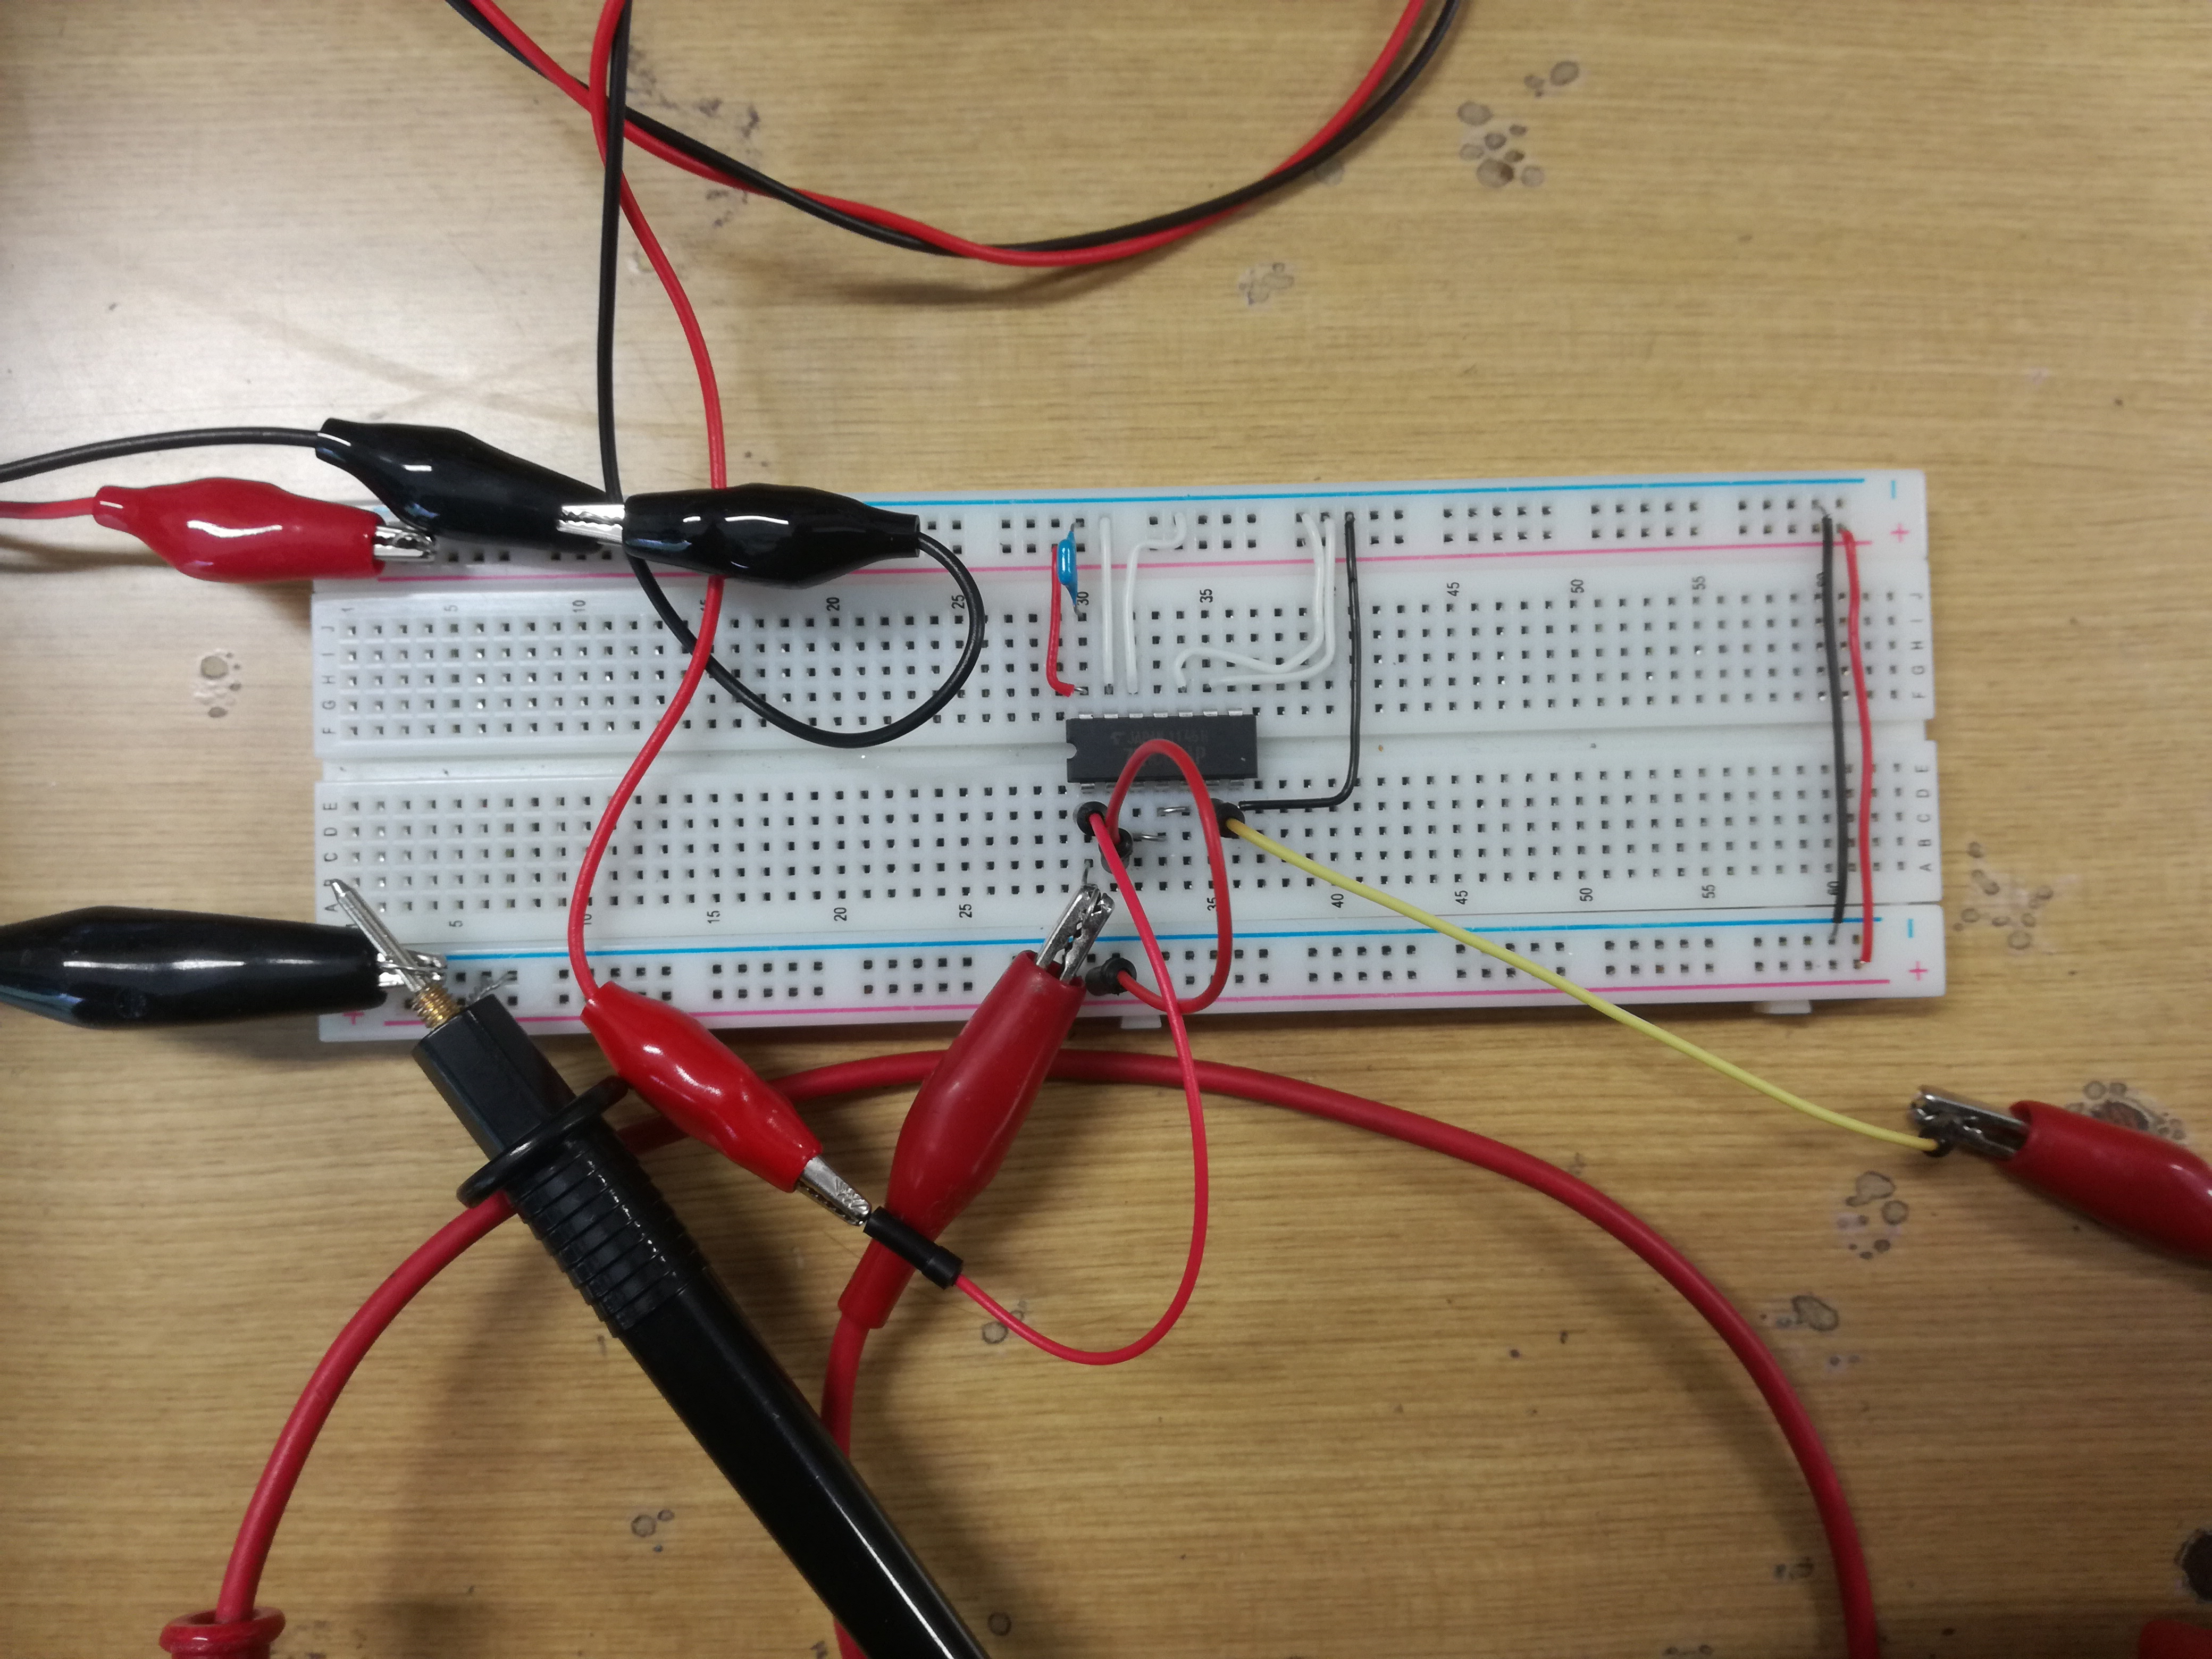
\includegraphics[width=0.8\hsize]{images/camera/7_1_camera.jpg}
    	\caption{制作した回路}
		\label{fig:7.1.camera}
  \end{minipage}
\end{figure}
\begin{figure}[H]
	\centering
	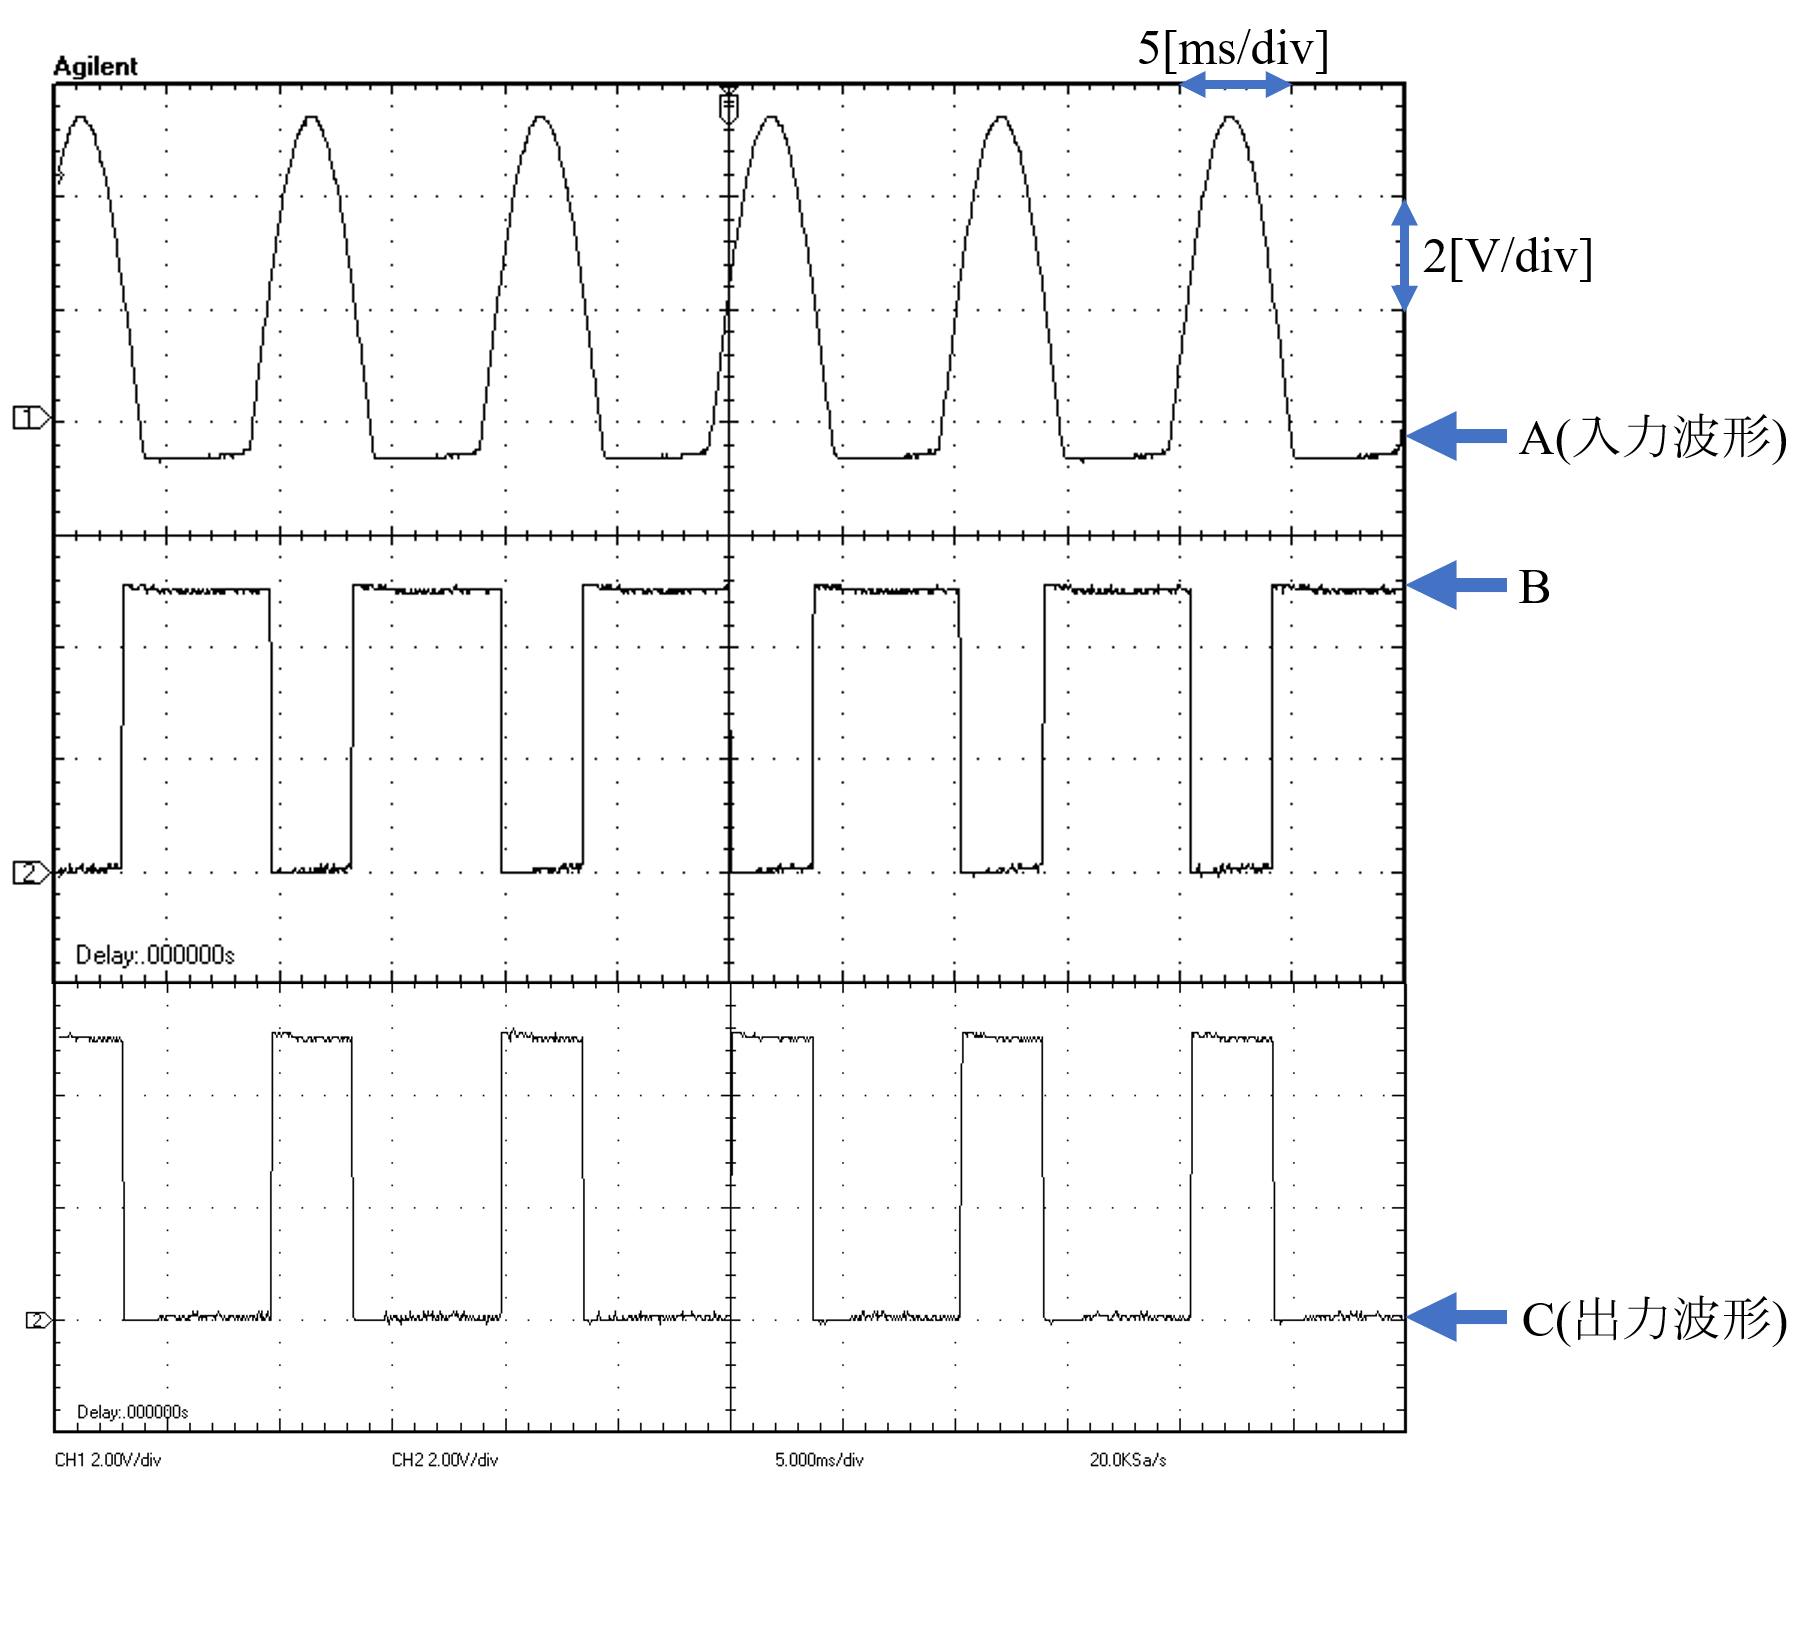
\includegraphics[width=0.8\hsize]{images/Experiment/7_1_graph.png}
	\caption{各部波形}
	\label{fig:7.1.graph}
\end{figure}
これらの結果から,実際に理想的な方形波は確認できないことが観察できる.
これは,IC内部のMOS-FETに逆電圧がかかることで空乏層が発生し,コンデンサとして回路中で働いてしまうことで,波形が変化していると考えられる.

\subsection{図4の動特性測定回路(波形整形回路(Schmitt回路))について,ダイオードの働きに注目して,この回路の動作を説明せよ.}
図4の回路の動作を各部に分けて考える.
\begin{enumerate}
	\item このとき,可変直流電源から入力された電圧は,それぞれ分岐して1つ目のNANDゲートに入る.
	\item 1つ目のNANDゲートに入力された電圧はNOTされ,2つ目のNANDゲートに入力される.
	\item 2つ目のNANDゲートによってNOTされた電圧は,分岐してダイオードと1つ目のNANDゲートの間に入力される.
	\item フィードバックされた電圧は,ダイオードによって行き先を制限され,1つ目のNANDゲートに入る.
\end{enumerate}
このとき,フィードバックされる電圧は抵抗によって減圧されている.
そのため,NANDゲートに入力される電圧の片方が閾値を超えず,結果として昇圧時には入力電圧が通常より大きい値にならなければ出力がHIGHにならない.
しかし,降圧時には入出力特性に影響がでないため,降圧時の閾値は通常のNANDゲートのものと大差ない結果となっている.

\subsection{図4の波形整形回路において,ダイオードを抵抗に置き換えても同様なヒステリシス特性を示し,その大きさは2つの抵抗比で決定される.それを実験により確認し,ダイオードの結果と比較し動作を説明せよ.また,ダイオードと置き換えた抵抗値の値について説明せよ.}
測定結果を次の図\ref{fig:7.3.graph}に示す.
\begin{figure}[H]
	\centering
	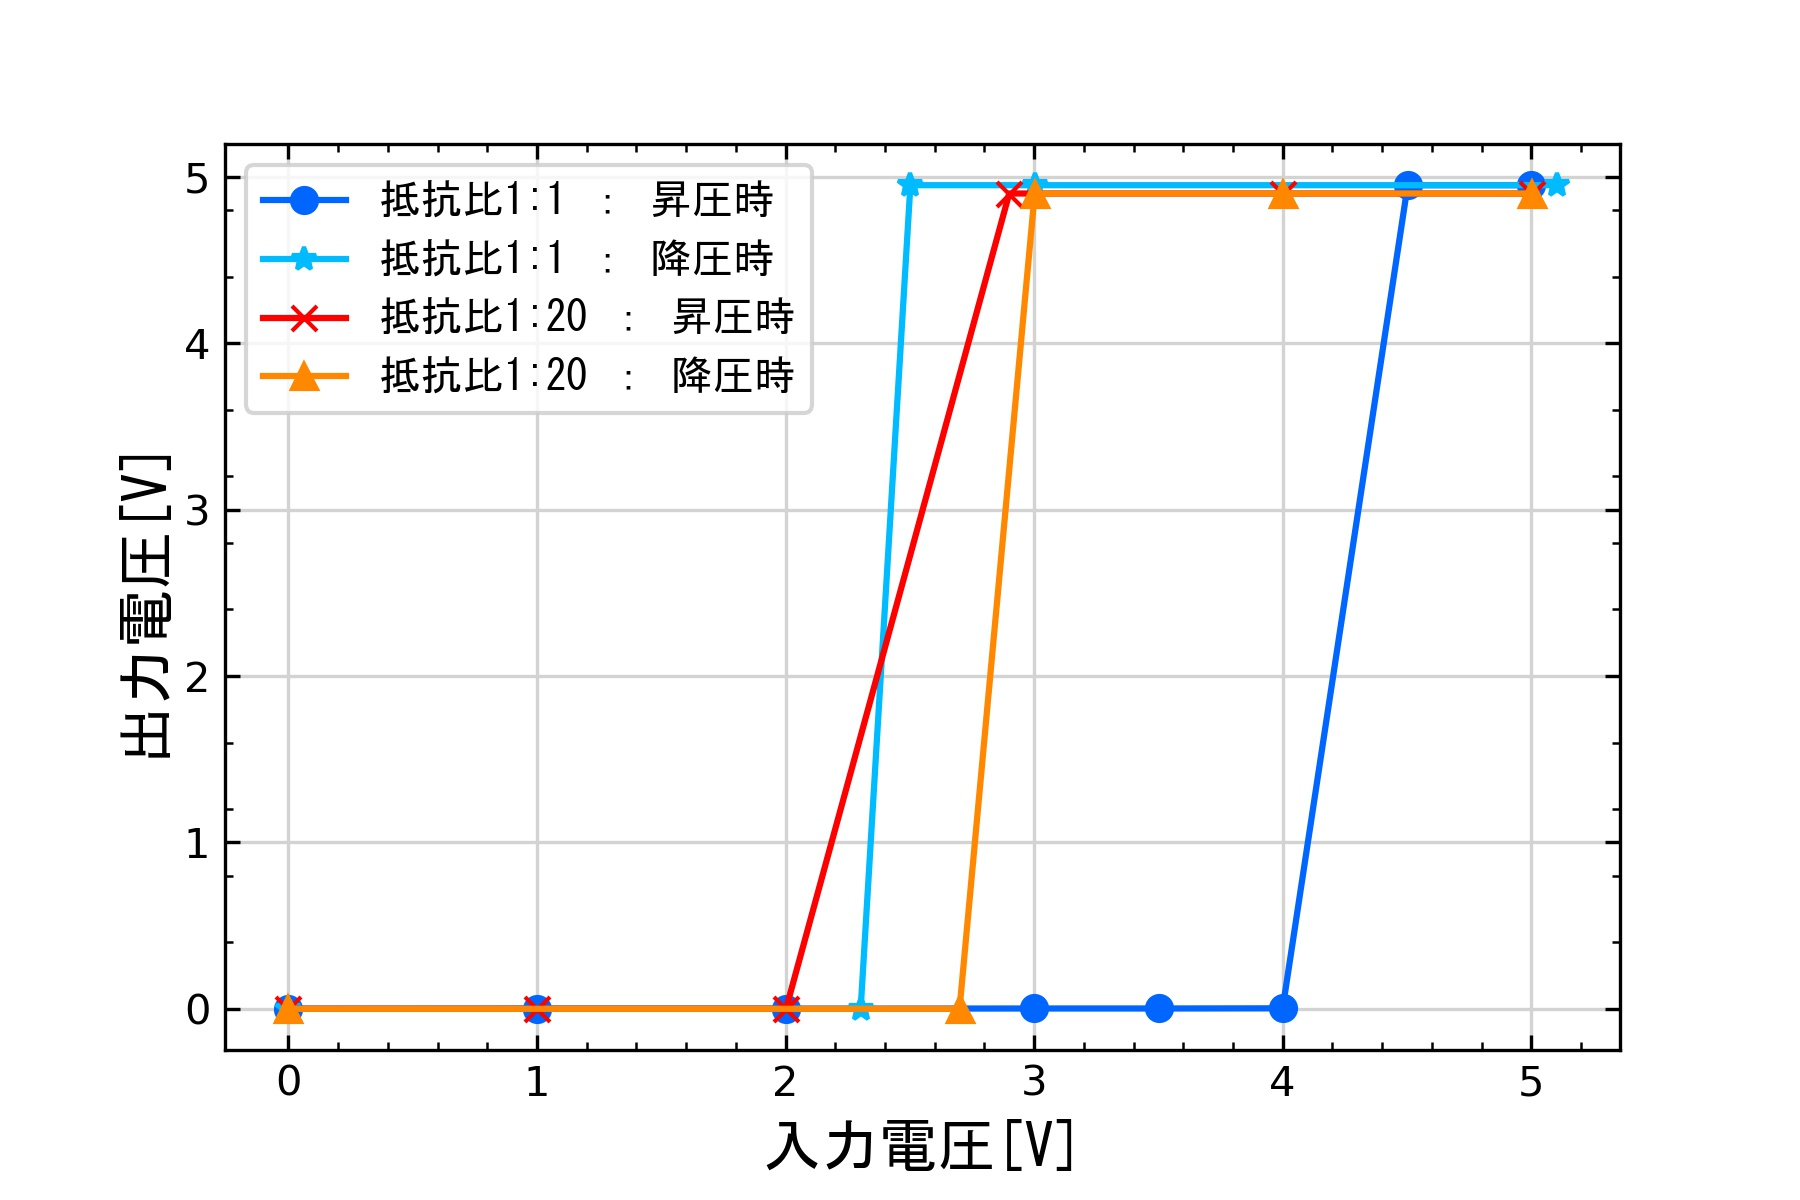
\includegraphics[width=0.8\hsize]{images/Experiment/7_3_graph.jpg}
	\caption{入力電圧と出力電圧の関係}
	\label{fig:7.3.graph}
\end{figure}
これらより,実際に題通りの特性を確認できる.

\subsection{TTLでは入力端子に500Ω程度以上の抵抗を接続することができない.この理由を説明せよ.}
これは,電流駆動型のTTLチップに大きな抵抗をつなぐと,電圧が非常に大きくなってしまうためである.


\section{参考文献}
\begin{enumerate}
	\item 標準ロジック アプリケーションノート\\ (URL:https://www.google.co.jp/url?sa=t\&rct=j\&q=\&esrc=s\&source=web\&cd=6\&ved=2ahUKEwinhOqImM3iAhXS62EKHVtBAcUQFjAFegQIBhAC\&url=https\%3A\%2F\%2Ftoshiba.semicon-storage.com\%2Finfo\%2Fdocget.jsp\%3Fdid\%3D12713\&usg=AOvVaw2MhXbXlXswO\_gtz8QOqvXO)
	\item デジタルICの基礎、組み合わせ回路\\(URL:https://www.renesas.com/jp/ja/support/technical-resources/engineer-school/digital-circuits-02-digital-ics-combinational-logic.html)
	\item TTL NAND回路\\(URL:http://www.ops.dti.ne.jp/~yanaka/digital/digital\_ic/1\_2\_purpose.html)
\end{enumerate}

\end{document}